% !TEX root = XRayMicroTomography.Presentation.tex
\usetheme[language=english]{ubbeamer2023}

\title{X-ray microtomography}
\subtitle{\href{https://ilias.unibe.ch/goto_ilias3_unibe_sess_3391298.html}{485018-HS2025-0: Advanced Course II Ultraprecision Engineering }}
\author{David Haberthür}
\institute{Institute of Anatomy}
\date{September 16, 2025}

%\includeonlyframes{current}
%then....
%\begin{frame}[label=current]
%\end{frame}

% Some often used abbreviations/commands
\newcommand{\everyframe}{1}% use only every nth frame for the animations
\newcommand{\imagewidth}{\linewidth}% set global image width
\newcommand{\standardimagewidth}{\linewidth}% Save us a standard image width, so we can always \renewcommand{\imagewidth} to it
\newcommand{\imageheight}{0.72\paperheight}% set global image height
\newcommand{\standardimageheight}{0.72\paperheight}% Save us standard image height, so we can always \renewommand{\imageheight} to it
\newlength\imagescale% needed for scalebars
\newcommand{\uct}{{\textmu}CT\xspace}% make our life easier
\newcommand{\eg}{e.\,g.\xspace}%
\newcommand{\ie}{i.\,e.\xspace}%

\usepackage[%
  backend=biber,%
  sorting=none,%
  %style=ieee,%
  citetracker=true,%
  isbn=false,%
  url=false,%
  maxnames=1,minnames=1,% Show only first author in references
]{biblatex}%
% Globally remove stuff from bibliography
% https://tex.stackexchange.com/a/25232
\DeclareSourcemap{%
  \maps[datatype=bibtex]{%
    \map{%
      \step[fieldset=journal, null]%
      \step[fieldset=editor, null]%
      \step[fieldset=volume, null]%
      \step[fieldset=number, null]%
      \step[fieldset=pages, null]%
      %\step[fieldset=year, null]% Do *not* remove year, otherwise the \citeyear on the history slide does not work :)
    }%
  }%
}%
\addbibresource{../../../../Documents/library.bib} % FastSSD, Windows or Mac works (on Linux/FastSSD we generated a 'Document' folder at the correct level and `ln -s ~/P/Documents/library.bib .` to it)
\usepackage{standalone}
\usepackage{tikz}
\usetikzlibrary{shadows,spy}
\tikzset{shadowed/.style={preaction={transform canvas={shift={(1pt,-1pt)}},draw=ubRed}}}
\usepackage{pgfplots}
\pgfplotsset{compat=1.18}
\usepackage{pgfplotstable}
\usepackage{shadowtext}
\shadowoffset{1pt}
\shadowcolor{ubRed}
\usepackage{microtype}
\usepackage[detect-all=true,
  range-phrase=--,
  range-units=single,
  per-mode=symbol,
per-symbol=/]{siunitx}
\usepackage[absolute,overlay]{textpos}
\usepackage[local]{gitinfo2}
\usepackage{xspace}
\usepackage{ccicons}
\usepackage[version=4]{mhchem}
\usepackage{animate}
\usepackage{fontawesome5}
\usepackage{csquotes}
\usepackage{listings}
\lstset{basicstyle=\scriptsize\ttfamily}
\usepackage{booktabs}
\renewcommand{\familydefault}{\rmdefault}
\usepackage[defaultmathsizes,symbolgreek]{mathastext}
\renewcommand{\familydefault}{\sfdefault}
\usepackage{colortbl}
\usepackage{multirow}
\usepackage[showseconds=false,showzone=false]{datetime2}
\usepackage[many]{tcolorbox}
\usepackage{hyperref}

% Define complementary colors to ubRed=e4003c, which is defined in the .sty file
% https://duckduckgo.com/?t=lm&q=html+e4003c&ia=answer
\definecolor{ubRedComplementary}{HTML}{00E3A6}

% change tikz font to slide font
% https://tex.stackexchange.com/a/33329/828
\usepackage[eulergreek]{sansmath}
\pgfplotsset{tick label style = {font=\sansmath\sffamily},
  every axis label = {font=\sansmath\sffamily},
  legend style = {font=\sansmath\sffamily},
  label style = {font=\sansmath\sffamily}
}

% Globally thicker lines in with tikz
% https://tex.stackexchange.com/a/206769/828
\tikzset{every picture/.style={thick}}

% Acknowledge images just below them
% Based on https://tex.stackexchange.com/a/282637/828
\newcommand{\source}[2]{%
  % Print out (short) link under image, with small text
  \raisebox{-1.618ex}{%
    \makebox[0pt][r]{%
      \tiny\href{http://#1}{#1} #2%
    }%
  }%
}%
\newcommand{\sourcecite}[2]{%
  % Cite (an image from) a reference
  \raisebox{-1.618ex}{%
    \makebox[0pt][r]{%
      \tiny From~\cite{#1}, #2%
    }%
  }%
}%
\newcommand{\sourcelink}[3]{%
  % Make the source command an \href{link}{text}
  \raisebox{-1.618ex}{%
    \makebox[0pt][r]{%
      \tiny\href{#1}{#2}, #3%
    }%
  }%
}%
\newcommand{\citeslide}[5]{% slideimage,lecturelink,lecturetitle,author,page
  % Drop a slide of another lecture into our presentation, with attribution
  \begin{tcolorbox}[enhanced,colframe=ubRed,colback=white,drop shadow,hbox,size=tight]{%
      \includegraphics[width=\linewidth,height=0.7\paperheight,keepaspectratio]{#1}% https://tex.stackexchange.com/a/12041/828
      \sourcelink{#2}{\emph{#3}, #4}{Slide #5}%
    }%
  \end{tcolorbox}%
}%

% Unobtrusive progress bar at the botton, based on 'update' in https://tex.stackexchange.com/a/554527/828
\makeatletter
\newdimen\progressbar@height%
\progressbar@height=1.36mm
% The template has "\put(15.2,-1.36){\usebeamercolor[fg]{ub page rule}\rule{\paperwidth-21.2mm}{1.36mm}}" for the header line, let's use this height as progressbar height
\addtobeamertemplate{footline}{}{%
  \mode<beamer>{%
    \begin{tikzpicture}%
      \useasboundingbox (0, \progressbar@height) rectangle (\paperwidth, \progressbar@height);%
      \draw[draw=ubRed, fill=white] (\insertframenumber/\inserttotalframenumber*\paperwidth, \progressbar@height) circle (\progressbar@height/2);%
    \end{tikzpicture}%
  }%
  \mode<handout>{\centering\tiny Handout for git.io/fjpP7, created on \DTMnow}%
}%
\makeatother

% Show current section at begin of sections, but only in presentation mode
\mode<beamer>{%
  \AtBeginSection[]{%
    \begin{frame}{Contents}%
      \tableofcontents[currentsection,currentsubsection,hideothersubsections]%
    \end{frame}%
  }%
}%

\begin{document}
\begin{frame}
  \maketitle
\end{frame}

\begin{frame}
	\frametitle{Grüessech mitenang!}
	\begin{itemize}
		\item David Haberthür
		\begin{itemize}
			\item Physicist by trade
			\item \href{https://boris.unibe.ch/2619/}{PhD in high resolution imaging of the lung}, Institute of Anatomy, University of Bern, Switzerland
			\item Post-Doc I: \href{https://www.psi.ch/sls/tomcat/}{TOMCAT}, \href{https://www.psi.ch/sls/}{Swiss Light Source}, \href{https://www.psi.ch/}{Paul Scherrer Institute}, Switzerland
			\item Post-Doc II: \uct group, Institute of Anatomy, University of Bern, Switzerland
		\end{itemize}
	\end{itemize}
\end{frame}

\begin{frame}
	\frametitle{Grüessech from the \uct group}
		\centering%
		\includegraphics[width=\imagewidth]{./images/team}
		\begin{columns}
		  \hfill%
		  \begin{column}{0.3\linewidth}
			David{\color{ubRed}.}Haberthuer{\color{ubRed}@unibe.ch}%
		  \end{column}%
		  \hfill%
		  \begin{column}{0.3\linewidth}
			Ruslan{\color{ubRed}.}Hlushchuk{\color{ubRed}@unibe.ch}%
		  \end{column}%
		  \hfill%
		  \begin{column}{0.3\linewidth}
			Oleksiy{\color{ubRed}.}Khoma{\color{ubRed}@unibe.ch}%
		  \end{column}%
		  \hfill%
		\end{columns}
	  \end{frame}

\begin{frame}
	\frametitle{\uct-group}
	\begin{columns}
		\begin{column}{0.62\linewidth}
			\begin{itemize}
				\item microangioCT~\cite{Hlushchuk2018}
				\begin{itemize}
					\item Angiogenesis: heart, musculature~\cite{Nording2021} and bones
					\item Vasculature: (mouse) brain~\cite{Hlushchuk2020}, (human) nerve scaffolds~\cite{Wuthrich2020}, (human) skin flaps~\cite{Zubler2021} and tumors
				\end{itemize}
				\item Zebrafish musculature and gills~\cite{MesserliAaldijk2020}
				\item (Lung) tumor detection and metastasis classification~\cite{Trappetti2021}
				\item Collaborations with museums~\cite{Bochud2021} and scientist at UniBe~\cite{Halm2021} to scan a wide range of specimens
				\item Automate \emph{all} the things!~\cite{Haberthuer2021, Haberthuer2023}
			\end{itemize}
		\end{column}%
		\begin{column}{0.38\linewidth}%
			\centering%
			\includegraphics<1|handout:0>[width=\imagewidth]{./images/1172}%
			\only<1|handout:0>{\source{brukersupport.com}{}}%
			\includegraphics<2|handout:1>[width=\imagewidth]{./images/1272}%
			\only<2|handout:1>{\source{bruker.com/skyscan1272}{}}%
			\includegraphics<3|handout:0>[width=\imagewidth]{./images/2214}%
			\only<3|handout:0>{\source{bruker.com/skyscan2214}{}}%
		\end{column}%
	\end{columns}%
\end{frame}

\begin{frame}{Contents}
	\tableofcontents
\end{frame}

\section{Overview \& Imaging methods}
\begin{frame}
	\frametitle{\uct}
	\begin{itemize}
		\item Dense and/or non‐transparent samples
		\item Calibrated \& isotropic 3D images at micron resolutions
		\item Covers a very large range of sample sizes
		\item Gives information at different length scales
		\item Nondestructive imaging, thus compatible with routine sample preparation.\newline
			Enables correlative imaging pipelines, scanning of museum \& collection material
	\end{itemize}
\end{frame}

\begin{frame}
	\frametitle{Biomedical imaging}%
	\begin{columns}
		\begin{column}{0.6\linewidth}%
			\begin{itemize}%
				\item<1-|handout:1-> Medical research%
				\item<1-|handout:1-> Non-destructive insights into the samples%
				\item<2-|handout:1-> (Small) Biological samples%
			\end{itemize}%
		\end{column}%
		\begin{column}{0.4\linewidth}%
			\centering%
			\only<1-2|handout:1>{%
				\includegraphics[width=\imagewidth]{./images/Sagittal_brain_MRI}%
				\source{w.wiki/7g4}{\ccbysa}%
			}%
			\only<3|handout:2>{%
				\begin{tikzpicture}[remember picture,overlay]%
					\node at (current page.center){%
						\mode<beamer>{\animategraphics[loop,autoplay,width=\paperwidth,every=\everyframe]{24}{./movies/mouse_skull/mouse_skull}{000}{236}}%
						\mode<handout>{\includegraphics[width=\paperwidth]{./movies/mouse_skull/mouse_skull075}}
					};%
				\end{tikzpicture}%
			}%
		\end{column}%
	\end{columns}%
\end{frame}

\begin{frame}
	\frametitle{Wavelengths \& Scales}
	\centering%
	\only<1|handout:1>{%
		\includegraphics[height=\imageheight]{./images/2000px-Electromagnetic_spectrum_with_sources}%
		\source{w.wiki/7fz}{\ccbysa}%
		}%
	\only<2|handout:2>{%
		\frame{\includegraphics[height=\imageheight]{./images/MIC-AM_techniques}}%
		\sourcelink{https://anatomie.unibe.ch/tschanz}{Stefan Tschanz}{with permission}%
		}%
\end{frame}

\begin{frame}
	\frametitle{Imaging methods}
	\begin{itemize}
		\item Light (sheet) microscopy: see \href{https://ilias.unibe.ch/goto_ilias3_unibe_sess_2177945.html}{lecture of Nadia Mercader Huber}
		\item X-ray imaging
		\item Electron microscopy
		\begin{itemize}
			\item \href{https://moodle.bfh.ch/course/section.php?id=546756}{\emph{Analytical electron microscopy} by Dimitri}
			\item \href{https://ilias.unibe.ch/goto_ilias3_unibe_sess_2177954.html}{\emph{SEM Grundlagen} by Sabine Kässmeyer and Ivana Jaric}
			\item \href{https://ilias.unibe.ch/goto_ilias3_unibe_sess_2177956.html}{\emph{Cryoelectron Microscopy \& Serial Block Face SEM} by Ioan}
		\end{itemize}
	\end{itemize}
\end{frame}

\section{Tomography}
\begin{frame}
	\frametitle{CT-Scanner}
	\centering%
	\mode<beamer>{%
		\animategraphics[loop,autoplay,height=\imageheight,every=\everyframe]{24}{./movies/ct-scanner/ct-scanner0}{001}{480}%
		\source{youtu.be/2CWpZKuy-NE}{}%
		}%
	\mode<handout>{%
		\includegraphics[height=\imageheight]{./movies/ct-scanner/ct-scanner0001}%
		\source{youtu.be/2CWpZKuy-NE}{}%
		}%
	\note{From \href{https://www.bruker.com/products/microtomography/micro-ct-for-sample-scanning/x-ray-micro-ct-microtomography.html}{Bruker Homepage}:
		Micro computed tomography or micro-CT is x-ray imaging in 3D, by the same method used in hospital CT (or CAT) scans, but on a small scale with massively increased resolution.
		It really represents 3D microscopy, where very fine scale internal structure of objects is imaged non-destructively.
		No sample preparation, no staining, no thin slicing - a single scan will image your sample's complete internal 3D structure at high resolution, plus you get your intact sample back at the end!}
\end{frame}

\subsection{History}
\begin{frame}
  \frametitle<1>{History}
  \frametitle<2->{CT History}
  \begin{columns}
    \begin{column}{0.49\linewidth}
      \begin{itemize}
        \item 1895: Wilhelm Conrad Röntgen discovers X-rays
        \item<2-|handout:2-> \citeyear{Cormack1963}:~\citeauthor{Cormack1963} used a collimated \ce{^{60}Co} source and a Geiger counter as a detector~\cite{Cormack1963}%
        \item<2-|handout:2-> \citeyear{Hounsfield1976a}:~\citeauthor{Hounsfield1976a} worked on first clinical scanner~\cite{Hounsfield1976a}%
        \item<3-|handout:3-> Nobel Prize in 1979, jointly for Allan Cormack and Godfrey Hounsfield
        \item<4-|handout:4-> CT scanner generations
          \begin{itemize}
            \item<4-|handout:4-> First generation
            \item<5-|handout:5-> Second generation
            \item<6|handout:6> Third generation
          \end{itemize}
      \end{itemize}
    \end{column}
    \begin{column}{0.49\linewidth}
      \centering%
      \includegraphics<1|handout:1>[height=\imageheight]{./images/First_medical_X-ray_by_Wilhelm_Röntgen_of_his_wife_Anna_Bertha_Ludwig's_hand_-_18951222}%
      \only<1|handout:1>{\source{w.wiki/BHAN}{\ccPublicDomain}}%
      \only<2|handout:2>{%
        \renewcommand{\imagewidth}{0.52\paperheight}% redefine imagewidth \only here so that we can use the simple way to draw a scale bar. 0.52 is an empirically found value
        \pgfmathsetlength{\imagescale}{\imagewidth/1055}%
        \def\x{652}% scalebar-x starting at golden ratio of image width of 1055px = 652
        \def\y{1328}% scalebar-y at 90% of image height of 1476px = 1328
        \begin{tikzpicture}[x=\imagescale,y=-\imagescale]
          \node[anchor=north west, inner sep=0pt, outer sep=0pt] at (0,0) {\includegraphics[width=\imagewidth]{./images/first_ct_image}};
          % 633.730px = 160.00000004mm -> 100px = 25247.344um -> 1.980px = 500um, 0.396px = 100um
          %\draw[|-|,blue,thick] (224,832) -- (858,826) node [sloped,midway,above,fill=white,semitransparent,text opacity=1] {\qty{160.00000004}{\milli\meter} (634px) TEMPORARY!};
          \draw[|-|,white,shadowed] (\x,\y) -- (\x+198.0,\y) node [midway,above] {\shadowtext{\qty{5}{\centi\meter}}};
        \end{tikzpicture}%
      }%
      \only<2|handout:2>{\sourcecite{Beckmann2006}{Figure 5}}%
      \includegraphics<3|handout:3>[height=\imageheight]{./images/US3940625-drawings-page-2}%
      \only<3|handout:3>{\sourcecite{US3940625A}{p.~2}}%
      \includegraphics<4|handout:4>[width=\imagewidth]{./images/History_Generation1}%
      \only<4|handout:4>{\sourcecite{Hsieh2003}{Figure 1.12}}%
      \includegraphics<5|handout:5>[width=\imagewidth]{./images/History_Generation2}%
      \only<5|handout:5>{\sourcecite{Hsieh2003}{Figure 1.13}}%
      \includegraphics<6|handout:6>[width=\imagewidth]{./images/History_Generation3}%
      \only<6|handout:6>{\sourcecite{Hsieh2003}{Figure 1.14}}%
    \end{column}
  \end{columns}
  \note<1|handout:1>{I was unable to find conclusive information on the voxel size of the first CT image.
    My head is approximately \qty{16}{\centi\meter} wide.
    I counted 47 voxels across the head in the image.
    This gives a voxel size of \qty{3.4}{\milli\meter} per voxel.}
  \note<4|handout:4>{Cone-beam MicroCT: A major development was the introduction of cone-beam microCT, which uses a cone-shaped X-ray beam and a flat-panel detector, allowing for faster image acquisition and higher resolution.
    In the late 1990s, Dr Yoshinori Arai in Japan and Dr Piero Mozzo in Italy independently developed Cone Beam Computed Technology for oral and maxillofacial radiology.
    The first commercial system (the NewTom 9000) was introduced in the European market in 1996 and into the US market in 2001, by Italian company Quantitative Radiology.}
\end{frame}
\renewcommand{\imagewidth}{\standardimagewidth}

\begin{frame}[allowframebreaks]
	\frametitle{\uct{} History}
	\begin{itemize}
	  \item X-ray computed tomography began to replace analog focal plane tomography in the early 1970s~\cite{Lin2019}
	  \item Non-medical use in the late 1970s, for detection of internal defects in fabricated parts and equipment
	  \item Lee Feldkamp~\cite{Feldkamp1984} developed an early laboratory microCT system by assembling a micro-focus cone beam x-ray source, specimen holder and stagers, and an image intensifier at Ford Motor Company’s Scientific Research Laboratory to nondestructively detect damage in ceramic manufactured automobile parts
	  \item Feldkamp met with scientists at Henry Ford Hospital and University of Michigan interested in understanding the relationship between the microstructure and biomechanical function of trabecular bone to study osteoporotic fractures~\cite{Feldkamp1983}
		\pagebreak
	  \item \uct{} was first reported in the 1980s, for scanning gemstones
	  \item Early 1990s: Manufacturers like SkyScan and Scanco Medical made \uct{} systems commercially available
	  \item Today: Nondestructive imaging for quantifying the (micro)structure of (organic) materials
		\begin{itemize}
		  \item Mineralized bone tissue and the relationships between the mechanical behavior of bone to its structural and compositional properties
		  \item Teeth and their internal details
		  \item Tissues, small animals, and medical devices like stents and implants
		  \item Soft tissues and vasculature using radio-opaque contrast agents
		  \item Characterization of anatomical details in high resolution
		\end{itemize}
	  \item \(\approx\)2500 \uct{} systems are in use worldwide with over 1000 publications annually
	\end{itemize}
  \end{frame}
  

\subsection{Interaction of x-rays with matter}
\begin{frame}
	\frametitle{X-ray interaction}
	\begin{itemize}
		\item \textquote[\cite{xrayphysics}]{X-rays interact with tissue in 2 main ways: photoelectric effect and Compton scatter.
				To a first approximation, the photoelectric effect contributes to contrast while the Compton effect contributes to noise.
				Both contribute to dose.}
		\begin{itemize}
			\item Photoelectric absorption (\(\tau\)) is strongly dependent on the atomic number \(Z\) of the absorbing material: \(\tau\propto\frac{Z^4}{E^{3.5}}\)
			\note{From \href{https://radiopaedia.org/articles/photoelectric-effect}{Radiopaedia.org}: Therefore if \(Z\) doubles, PEA will increase by a factor of 16 (\(2^4=16\)), and if \(E\) doubles PEA will be reduced by a factor of 11.
<				Small changes in \(Z\) and \(E\) can therefore significantly affect PEA\@.
				This has practical implications in the field of radiation protection and is the reason why materials with a high \(Z\) such as lead (\(Z= 82\)) are useful shielding materials.
				The dependence of PEA on \(Z\) and \(E\) means that it is the major contributor to beam attenuation up to approximately \qty{30}{\kilo\electronvolt} when human tissues (\(Z=7.4\)) are irradiated.
				At beam energies above this, the Compton effect predominates.}
			\item Compton scattering is one of the principle forms of photon interaction and is directly proportional to the (electron \& physical) density of the material.
				It does \emph{not} depend on the atomic number: \(\lambda' - \lambda = \frac{h}{m_e c}\left(1-\cos{\theta}\right)\)
			\note{Where \(\lambda\) is the initial wavelength, \(\lambda'\) is the wavelength after scattering, \(h\) is the Planck constant, \(m_e\) is the electron rest mass, \(c\) is the speed of light, and \(\theta\) is the scattering angle.}
		\end{itemize}
		\item Lowering x-ray energy increases contrast
		\item X-ray penetration decreases exponentially with sample thickness~\cite[\ie Beer-Lamberts law]{wiki:beer-lambert}: \(I(t) = I_0 \, e^{-\alpha z}\)
	\end{itemize}
\end{frame}

\begin{frame}
	\frametitle{Composition of biological tissues}
	Tissue: content by mass percentage
	\centering
	\begin{table}%
	  \only<1|handout:0>{%
		\pgfplotstabletypeset[%
		  col sep=comma,% the seperator in our .csv file
		  display columns/0/.style={string type},%
		  % section 3.2 in pgfplotstable manual
		  every head row/.style={before row={\toprule}},%
		  every row no 0/.style={after row=\midrule},%
		  every last row/.style={after row=\bottomrule},%
		]{./tables/tissue-composition.csv}%
	  }%
	  \only<2|handout:1>{%
		\pgfplotstabletypeset[%
		  col sep=comma,% the seperator in our .csv file
		  display columns/0/.style={string type},%
		  every head row/.style={before row={\toprule}},%
		  every row no 0/.style={after row=\midrule},%
		  every last row/.style={after row=\bottomrule},%
		  % make certain cells ubRed, based on https://tex.stackexchange.com/a/296914/828
		  every row 1 column 2/.style={postproc cell content/.append style={/pgfplots/table/@cell content/.add={\cellcolor{ubRed!61.8}}{}}},%
		  every row 2 column 4/.style={postproc cell content/.append style={/pgfplots/table/@cell content/.add={\cellcolor{ubRed!61.8}}{}}},%
		  every row 3 column 4/.style={postproc cell content/.append style={/pgfplots/table/@cell content/.add={\cellcolor{ubRed!61.8}}{}}},%
		  every row 4 column 4/.style={postproc cell content/.append style={/pgfplots/table/@cell content/.add={\cellcolor{ubRed!61.8}}{}}},%
		  every row 5 column 4/.style={postproc cell content/.append style={/pgfplots/table/@cell content/.add={\cellcolor{ubRed!61.8}}{}}},%
		  every row 6 column 6/.style={postproc cell content/.append style={/pgfplots/table/@cell content/.add={\cellcolor{ubRed!61.8}}{}}},%
		  every row 6 column 10/.style={postproc cell content/.append style={/pgfplots/table/@cell content/.add={\cellcolor{ubRed!61.8}}{}}}%
		]{./tables/tissue-composition.csv}%
	  }%
	\end{table}
	\note{In an \emph{unstained} sample, bone, lean tissue, fat and air can be distinguished easily}
  \end{frame}

\begin{frame}
	\frametitle{Why \uct?}
	\begin{columns}
		\begin{column}{0.49\linewidth}% deliberately a bit smaller here, so that the images do not touch
			\centering%
			% https://www.cancerimagingarchive.net/nbia-search/?saved-cart=nbia-76761575299081509
			\only<1-4|handout:1-4>{%
				\pgfmathsetlength{\imagescale}{\imagewidth/512}%
				\def\x{316}% scalebar-x starting at golden ratio of image width of 512px = 316
				\def\y{361}% scalebar-y at 90% of image height of 401px = 361
				\begin{tikzpicture}[x=\imagescale,y=-\imagescale]
					\node[anchor=north west, inner sep=0pt, outer sep=0pt] at (0,0) {\includegraphics[width=\imagewidth]{./images/comparison/MAX_human}};
					% 512.000px = 250.0096mm -> 100px = 48830.000um -> 1.024px = 500um, 0.205px = 100um
					%\draw[|-|,blue,thick] (0,200) -- (512,200) node [sloped,midway,above,fill=white,semitransparent,text opacity=1] {\qty{250.0096}{\milli\meter} (512px) TEMPORARY!};
					\draw[|-|,white,shadowed] (\x,\y) -- (\x+102.4,\y) node [midway,above] {\shadowtext{\qty{5}{\centi\meter}}};
				\end{tikzpicture}%
			}%
			\only<5|handout:0>{%
				\pgfmathsetlength{\imagescale}{\imagewidth/512}%
				\def\x{316}% scalebar-x starting at golden ratio of image width of 512px = 316
				\def\y{361}% scalebar-y at 90% of image height of 401px = 361
				\def\mag{5}% magnification of inset
				\def\size{100}% size of inset
				\begin{tikzpicture}[x=\imagescale,y=-\imagescale,spy using outlines={rectangle,magnification=\mag,size=\size,connect spies}]
					\node[anchor=north west, inner sep=0pt, outer sep=0pt] at (0,0) {\includegraphics[width=\imagewidth]{./images/comparison/MAX_human}};
					\spy [red] on (102,342) in node at (256,201) [anchor=center];
					% 512.000px = 250.0096mm -> 100px = 48830.000um -> 1.024px = 500um, 0.205px = 100um
					\draw[|-|,white,shadowed] (\x,\y) -- (\x+102.4,\y) node [midway,above] {\shadowtext{\qty{5}{\centi\meter}}};
				\end{tikzpicture}%
			}%
			\only<6|handout:5>{%
				\renewcommand{\imagewidth}{0.1554\linewidth}% redefine the width only locally
				\pgfmathsetlength{\imagescale}{\imagewidth/512}%
				\def\x{316}% scalebar-x starting at golden ratio of image width of 512px = 316
				\def\y{361}% scalebar-y at 90% of image height of 401px = 361
				\begin{tikzpicture}[x=\imagescale,y=-\imagescale]
					\node[anchor=north west, inner sep=0pt, outer sep=0pt] at (0,0) {\includegraphics[width=\imagewidth]{./images/comparison/MAX_human}};
					% 512.000px = 250.0096mm -> 100px = 48830.000um -> 1.024px = 500um, 0.205px = 100um
					\draw[|-|,white,shadowed] (\x,\y) -- (\x+102.4,\y) node [midway,above] {\shadowtext{\qty{5}{\centi\meter}}};
				\end{tikzpicture}%
			}%
			\sourcecite{Clark2013}{Subject \emph{C3L-02465}}
		\end{column}%
		\begin{column}{0.49\linewidth}% deliberately a bit smaller here, so that the images do not touch
			\centering%
			\only<1|handout:1>{%
				\pgfmathsetlength{\imagescale}{\imagewidth/3295}%
				\def\x{2036}% scalebar-x starting at golden ratio of image width of 3295px = 2036
				\def\y{1343}% scalebar-y at 90% of image height of 1492px = 1343
				\begin{tikzpicture}[x=\imagescale,y=-\imagescale]
					\node[anchor=north west, inner sep=0pt, outer sep=0pt] at (0,0) {\includegraphics[width=\imagewidth]{./images/comparison/MAX_mouse}};
					% 3295.000px = 26.2282mm -> 100px = 796.000um -> 62.814px = 500um, 12.563px = 100um
					%\draw[|-|,blue,thick] (0,746) -- (3295,746) node [sloped,midway,above,fill=white,semitransparent,text opacity=1] {\qty{26.2282}{\milli\meter} (3295px) TEMPORARY!};
					\draw[|-|,white,shadowed] (\x,\y) -- (\x+628.14,\y) node [midway,above] {\shadowtext{\qty{5}{\milli\meter}}};
				\end{tikzpicture}%
			}%
			\only<2|handout:2>{%
				\renewcommand{\imagewidth}{0.1\columnwidth}%
				\pgfmathsetlength{\imagescale}{\imagewidth/54}%
				\def\x{33}% scalebar-x starting at golden ratio of image width of 54px = 33
				\def\y{22}% scalebar-y at 90% of image height of 24px = 22
				\begin{tikzpicture}[x=\imagescale,y=-\imagescale]
					\node[anchor=north west, inner sep=0pt, outer sep=0pt] at (0,0) {\includegraphics[width=\imagewidth]{./images/comparison/MAX_mouse_488umppx}};
					% 54.000px = 26.3682mm -> 100px = 48830.000um -> 1.024px = 500um, 0.205px = 100um
					%\draw[|-|,blue,thick] (0,12) -- (54,12) node [sloped,midway,above,fill=white,semitransparent,text opacity=1] {\qty{26.3682}{\milli\meter} (54px) TEMPORARY!};
					\draw[|-|,white,shadowed] (\x,\y) -- (\x+102.4,\y) node [midway,above] {\shadowtext{\qty{5}{\centi\meter}}};
					%\draw[color=red, anchor=south west] (0,24) node [fill=white, semitransparent] {Legend} node {Legend};
				\end{tikzpicture}%
			}%
			\only<3|handout:3>{%
				\renewcommand{\imagewidth}{\columnwidth}%
				\pgfmathsetlength{\imagescale}{\imagewidth/54}%
				\def\x{33}% scalebar-x starting at golden ratio of image width of 54px = 33
				\def\y{22}% scalebar-y at 90% of image height of 24px = 22
				\begin{tikzpicture}[x=\imagescale,y=-\imagescale]
					\node[anchor=north west, inner sep=0pt, outer sep=0pt] at (0,0) {\includegraphics[width=\imagewidth]{./images/comparison/MAX_mouse_488umppx}};
					% 54.000px = 26.3682mm -> 100px = 48830.000um -> 1.024px = 500um, 0.205px = 100um
					%\draw[|-|,blue,thick] (0,12) -- (54,12) node [sloped,midway,above,fill=white,semitransparent,text opacity=1] {\qty{26.3682}{\milli\meter} (54px) TEMPORARY!};
					\draw[|-|,white,shadowed] (\x,\y) -- (\x+10.24,\y) node [midway,above] {\shadowtext{\qty{5}{\milli\meter}}};
					%\draw[color=red, anchor=south west] (0,24) node [fill=white, semitransparent] {Legend} node {Legend};
				\end{tikzpicture}%
			}%
			\only<4|handout:4>{%
				\pgfmathsetlength{\imagescale}{\imagewidth/3295}%
				\def\x{2036}% scalebar-x starting at golden ratio of image width of 3295px = 2036
				\def\y{1343}% scalebar-y at 90% of image height of 1492px = 1343
				\begin{tikzpicture}[x=\imagescale,y=-\imagescale]
					\node[anchor=north west, inner sep=0pt, outer sep=0pt] at (0,0) {\includegraphics[width=\imagewidth]{./images/comparison/MAX_mouse}};
					% 3295.000px = 26.2282mm -> 100px = 796.000um -> 62.814px = 500um, 12.563px = 100um
					\draw[|-|,white,shadowed] (\x,\y) -- (\x+628.14,\y) node [midway,above] {\shadowtext{\qty{5}{\milli\meter}}};
				\end{tikzpicture}%
			}%
			\only<5|handout:0>{%
				\pgfmathsetlength{\imagescale}{\imagewidth/3295}%
				\def\x{2036}% scalebar-x starting at golden ratio of image width of 3295px = 2036
				\def\y{1343}% scalebar-y at 90% of image height of 1492px = 1343
				\def\mag{5}% magnification of inset
				\def\size{100}% size of inset
				\begin{tikzpicture}[x=\imagescale,y=-\imagescale,spy using outlines={rectangle,magnification=\mag,size=\size,connect spies}]
					\node[anchor=north west, inner sep=0pt, outer sep=0pt] at (0,0) {\includegraphics[width=\imagewidth]{./images/comparison/MAX_mouse}};
					\spy [red] on (352,1116) in node at (1648,746) [anchor=center];
					% 3295.000px = 26.2282mm -> 100px = 796.000um -> 62.814px = 500um, 12.563px = 100um
					\draw[|-|,white,shadowed] (\x,\y) -- (\x+628.14,\y) node [midway,above] {\shadowtext{\qty{5}{\milli\meter}}};
				\end{tikzpicture}%
			}%
			\only<6|handout:5>{%
				\pgfmathsetlength{\imagescale}{\imagewidth/3295}%
				\def\x{2036}% scalebar-x starting at golden ratio of image width of 3295px = 2036
				\def\y{1343}% scalebar-y at 90% of image height of 1492px = 1343
				\begin{tikzpicture}[x=\imagescale,y=-\imagescale]
					\node[anchor=north west, inner sep=0pt, outer sep=0pt] at (0,0) {\includegraphics[width=\imagewidth]{./images/comparison/MAX_mouse}};
					% 3295.000px = 26.2282mm -> 100px = 796.000um -> 62.814px = 500um, 12.563px = 100um
					\draw[|-|,white,shadowed] (\x,\y) -- (\x+628.14,\y) node [midway,above] {\shadowtext{\qty{5}{\milli\meter}}};
				\end{tikzpicture}%
			}%
		\end{column}
	\end{columns}
	\note<1|handout:1>{The human head scan was downloaded from the \href{https://www.cancerimagingarchive.net}{Cancer Imaging Archive}.
		We loaded the DICOM slices in Fiji, resliced it to show it from the side and then used to generate an MIP\@.
		According to the DICOM tags, the voxel size is \qtyproduct{0.4883 x 0.4883 x 0.625}{\milli\meter\cubed}, the image size is \numproduct{512 x 512} pixels.
		The mouse head is the same as shown in the early animation.
		The files from the early animation were resized 0.25 times; here we used the original dataset (Mouse1265\_Skull\_Gaby\_TKI\_7\_96um\_Al05\_2K) for a reslice and the generation of the MIP\@.
		The voxel size of the original data is \qty{7.96}{\micro\meter}, the image size is \numproduct{3295 x 1492} pixels.}
\end{frame}

\begin{frame}
	\frametitle{Maximum intensity projection}
	\centering%
	% pdfseparate 220923_Fundamentals_image_processing_2022_Witz.pdf -f 23 -l 23 220923_Fundamentals_image_processing_2022_Witz-%d.pdf
	\frame{\includegraphics[height=\imageheight]{./images/220923_Fundamentals_image_processing_2022_Witz-23}}
	\sourcelink{ilias.unibe.ch/goto_ilias3_unibe_sess_2466919.html}{\emph{Fundamentals of Digital Image Processing (2022)} by Guillaume Witz}{Slide 23}
\end{frame}

\subsection{Tomography today}
\begin{frame}
	\frametitle{Machinery}
	\begin{columns}
		\begin{column}{0.5\linewidth}%
			\begin{itemize}%
				\item<1-> Hospital CT%
				\begin{itemize}%
					\item Voxel size around \qty{0.5}{\milli\meter}%
				\end{itemize}%
				\item<2-> Lab/Desktop CT%
				\begin{itemize}%
					\item Voxel size around \qty{7}{\micro\meter} (\emph{in vivo})%
					\item Voxel size around \qty{0.5}{\micro\meter} (\emph{ex vivo})%
				\end{itemize}%
				\item<4-> Synchrotron CT%
				\begin{itemize}%
					\item Voxel size down to \href{https://www.psi.ch/en/sls/tomcat/detectors}{\qty{160}{\nano\meter}}%
				\end{itemize}%
			\end{itemize}%
		\end{column}%
		\begin{column}{0.5\linewidth}%
			\centering%
			\includegraphics<1|handout:1>[width=\imagewidth]{./images/24324062640_751e011e1a_o}%
			\only<1|handout:1>{\source{flic.kr/p/D4rbom}{\ccbyncsa}}%
			\includegraphics<2|handout:2>[height=\imageheight]{./images/9459311320_516179207a_o}%
			\only<2|handout:2>{\source{flic.kr/p/fpTrGu}{\ccbysa}}%
			\includegraphics<3|handout:3>[width=\imagewidth]{./images/1272}%
			\only<3|handout:3>{\source{bruker.com/skyscan1272}{}}%
			\includegraphics<4|handout:4>[width=\imagewidth]{./images/4563733710_f632792416_b}%
			\only<4|handout:4>{\source{flic.kr/p/7Xhk2Y}{\ccbync}}%
			%trim={<left> <lower> <right> <upper>}
			\includegraphics<5|handout:0>[trim={430 0 290 0},clip,width=\imagewidth]{./images/4563733710_f632792416_b}%
			\only<5|handout:0>{\source{flic.kr/p/7Xhk2Y}{\ccbync}}%
		\end{column}%
	\end{columns}%
	\note<1|handout:1>{Fan beam \textrightarrow Bruker and other \uct machines\newline
		Parallel beam \textrightarrow TOMCAT et al.\newline
		Helical/spiral CT/multislice CT \textrightarrow Hospitals}
\end{frame}

\renewcommand{\imagewidth}{\linewidth}
\begin{frame}
	\frametitle{What is happening?}
	\begin{columns}
		\begin{column}{0.5\linewidth}%
			No matter what kind of machine, the basic principle is always
			\begin{itemize}
				\item an x-ray source
				\item a sample
				\item a detector
			\end{itemize}
		\end{column}%
		\begin{column}{0.5\linewidth}%
			\centering%
			\includegraphics[width=\imagewidth]{./images/3D_Computed_Tomography}%
			\source{w.wiki/7g3}{\ccbysa}%
		\end{column}%
	\end{columns}%
\end{frame}

\begin{frame}
	\frametitle{Machinery}
	\begin{columns}
	  \begin{column}{0.5\textwidth}
		\centering
		%\documentclass{beamer}% For self-contained compilation
\documentclass[tikz]{standalone}% For inclusion in the presentation
% Draw the setup where the source and detector move, e.g. classic CT
% With help from https://tex.stackexchange.com/q/515519/828
\usepackage{animate}
\usepackage{tikz}
%	\usetikzlibrary{external}
%	\tikzexternalize
%	\tikzsetnextfilename{classicCT}
\usepackage{fontawesome5}
\usepackage{ifthen}
\ifthenelse{\isundefined{\everyframe}}{%
	% If we're compiling this file via \input, then these variables are already defined.
	% In the other case, we need to define them
	\newcommand{\everyframe}{5}
	\definecolor{ubRed}{HTML}{e4003c}%
	\definecolor{ubGrey}{HTML}{646363}%
	% split complementary images from https://www.sessions.edu/color-calculator/
	\definecolor{ubRedComplementary}{HTML}{2EE600}
	}{}
\begin{document}
\begin{animateinline}[loop,every=\everyframe]{25}
	\multiframe{90}{n=1+4}{%
		\begin{tikzpicture}[scale=1.618]
			\pgfdeclarelayer{background}
			\pgfsetlayers{background,main}
			\mode<beamer>{%
				%Help lines, to force same size of images
				\begin{pgfonlayer}{background}
					\draw[ubGrey,transparent] (-2.25,0) -- (2.25,0);
					\draw[ubGrey,transparent] (0,-2.25) -- (0,2.25);
					\draw[ubGrey,transparent,help lines,step=1cm,ultra thin] (-2.45,-2.45) grid (2.45,2.45);
				\end{pgfonlayer}
			}%
			% Stuff that stays put
			\node[ubRedComplementary] at (0,0) (sample) {\fontsize{64}{60}\selectfont \faUser};% Large patient: https://tex.stackexchange.com/a/716/828
			% Stuff that moves
			\begin{scope}[rotate around={\n:(sample)}]
				% Rotation arc
				\draw[->, thick,line cap=rect] (1.5,0) arc [start angle=0, end angle=180, radius=1.5];
				\draw[->, thick,line cap=rect] (-1.5,0) arc [start angle=-180, end angle=0, radius=1.5];
				% Source
				\fill[red] (-0.25,1.5) rectangle node (source) {} +(0.5,0.5);
				\draw[fill=yellow] (0,1.75) circle (0.2);
				\node at (0,1.735) (radiation) {\faRadiation};
				% Detector and detector edges
				\fill[ubGrey] (-0.5,-1.75) rectangle node (detector) {} +(1,0.25);
				\coordinate (dl) at (-0.45,-1.75);
				\coordinate (dr) at (0.45,-1.75);
				% X-ray cone
				\begin{pgfonlayer}{background}
					\fill[ubGrey, semitransparent] (source.center) -- (dl) -- (dr) -- cycle;
				\end{pgfonlayer}
			\end{scope}
		\end{tikzpicture}
	}
\end{animateinline}
\end{document}

		\pause
	  \end{column}
	  \begin{column}{0.5\textwidth}
		\centering
  		% "List" the LR, normal and HR animations in a weird order here, to display them nicely in the handout
  		\only<3|handout:1>{\documentclass{standalone}
% Draw the setup where the only the sample moves, e.g. microCT
% Essentially just a copy of classicCT in the same folder
\usepackage{animate}
\usepackage{tikz}
%	\usetikzlibrary{external}
%	\tikzexternalize
%	\tikzsetnextfilename{microCT}
\usepackage{fontawesome5}	
\usepackage{ifthen}
\ifthenelse{\isundefined{\everyframe}}{%
	% If we're compiling this file via \input, then these variables are already defined.
	% In the other case, we need to define them
	\newcommand{\everyframe}{5}
	\definecolor{ubRed}{HTML}{E6002E}
	% split complementary images from https://www.sessions.edu/color-calculator/
	\definecolor{ubRedComplementary1}{HTML}{00a1e6}
	\definecolor{ubRedComplementary2}{HTML}{00e645}
	\definecolor{ubGrey}{RGB}{217,217,217}
	}{}
\begin{document}
\begin{animateinline}[every=\everyframe,loop]{25}
	\multiframe{180}{n=1+2}{%
%	\tikzifexternalizing{Work-around to make animate happy	}{}%https://tex.stackexchange.com/a/39026/828
		\begin{tikzpicture}
			\pgfdeclarelayer{background}
			\pgfsetlayers{background,main}
			%Help lines
			\draw[<->] (-2.25,0) -- (2.25,0);
			\draw[<->] (0,-2.25) -- (0,2.25);
			\draw[help lines,step=1cm,ultra thin] (-2.45,-2.45) grid (2.45,2.45);
			% Stuff that stays put
			% Source
			\fill[ubRed] (-0.25,1) rectangle node (source) [black,opacity=0, text opacity=1] {X-ray} +(0.5,0.5);
			% Detector and detector edges
			\fill[ubRedComplementary2,fill] (-0.5,-1.25) rectangle node (detector) [black] {Detector} +(1,0.25);
			\coordinate (dl) at (-0.45,-1);
			\coordinate (dr) at (0.45,-1);
			% X-ray cone
			\begin{pgfonlayer}{background}
				\fill[gray,semitransparent] (source.center) -- (dl) -- (dr) -- cycle;
			\end{pgfonlayer}
			% Stuff that moves
			\mode<beamer>{%
				\begin{scope}[rotate around={\n:(0,-0.5)}]
				}
				% Rotation arc
				\draw[->, thick,line cap=rect] (0.618,-0.5) arc [start angle=0, end angle=180, radius=0.618];
				\draw[->, thick,line cap=rect] (-0.618,-0.5) arc [start angle=-180, end angle=0, radius=0.618];
				% Sample
				\node[ubRedComplementary1] at (0,-0.5) (sample) {\rotatebox{\n}{\huge\faFish}};
			\mode<beamer>{%
				\end{scope}
				}
		\end{tikzpicture}
	}
\end{animateinline}
\end{document}
}%
  		\only<1-2|handout:1>{\documentclass{standalone}%
% Draw the setup where the source and detector move, e.g. classic CT
% With help from https://tex.stackexchange.com/q/515519/828
\usepackage{fontawesome5}
\usepackage{ifthen}
\ifthenelse{\isundefined{\everyframe}}{%
	% If we're compiling this file via \input, then we already defined some things
	% In the other case, we need to define them
	\usepackage{tikz}
	\usepackage{animate}
	\newcommand{\everyframe}{5}
	\definecolor{ubRed}{HTML}{e4003c}%
	\definecolor{ubGrey}{HTML}{646363}%
	% split complementary images from https://www.sessions.edu/color-calculator/
	\definecolor{ubRedComplementary}{HTML}{2EE600}
	}{}
\begin{document}
\begin{animateinline}[loop,every=\everyframe]{25}
	\multiframe{90}{n=1+4}{%
		\begin{tikzpicture}[scale=1.25]
			\pgfdeclarelayer{background}
			\pgfsetlayers{background,main}
			%Help lines used to setup the animation (set to semitransparent), drawing them transparent in the presentation forces a consistent size
			\begin{pgfonlayer}{background}
				\draw[ubGrey,transparent,help lines,step=5mm] (-0.75,-1.25) grid (0.75,1.5);
			\end{pgfonlayer}
			% Stuff that stays put
			% Source
			\fill[ubRed] (-0.25,1) rectangle node (source) {} +(0.5,0.5);
			\draw[fill=yellow] (0,1.25) circle (0.2);
			\node at (0,1.235) (radiation) {\small\faRadiation};
			% Detector and detector edges
			\fill[gray] (-0.5,-1.25) rectangle node (detector) {} +(1,0.25);
			\coordinate (dl) at (-0.45,-1);
			\coordinate (dr) at (0.45,-1);
			% X-ray cone
			\begin{pgfonlayer}{background}
				\fill[gray,semitransparent] (source.center) -- (dl) -- (dr) -- cycle;
			\end{pgfonlayer}
			% Stuff that moves
				\begin{scope}[rotate around={\n:(0,0)}]
				% Rotation arc
				\draw[->, thick,line cap=rect] (0.618,0) arc [start angle=0, end angle=180, radius=0.618];
				\draw[->, thick,line cap=rect] (-0.618,0) arc [start angle=-180, end angle=0, radius=0.618];
				% Sample
				\node[ubRedComplementary] at (0,0) (sample) {\rotatebox{\n}{\normalsize\faFish}};
				\end{scope}
		\end{tikzpicture}
	}
\end{animateinline}
\end{document}
}%
  		\only<4|handout:1>{\documentclass{standalone}
% Draw the setup where the only the sample moves, e.g. microCT
% For the case of small samples close to the source
\usepackage{animate}
\usepackage{tikz}
\usepackage{pgf-pie}
\usepackage{fontawesome5}
\usepackage{ifthen}
\ifthenelse{\isundefined{\everyframe}}{%
	% If we're compiling this file via \input, then these variables are already defined.
	% In the other case, we need to define them
	\newcommand{\everyframe}{5}
	\definecolor{ubRed}{HTML}{E6002E}
	% complementary colors from https://www.sessions.edu/color-calculator/
	\definecolor{ubRedComplementary}{HTML}{2EE600}
	}{}
\begin{document}
\begin{animateinline}[every=\everyframe]{25}
	\multiframe{180}{n=1+2}{%
		\begin{tikzpicture}
			\pgfdeclarelayer{background}
			\pgfsetlayers{background,main}
			%Help lines
			%\draw[<->] (-2.25,0) -- (2.25,0);
			%\draw[<->] (0,-2.25) -- (0,2.25);
			%\draw[help lines,step=1cm,ultra thin] (-2.45,-2.45) grid (2.45,2.45);%
			% Stuff that stays put
			% X-ray source
			\fill[ubRed] (-0.25,1) rectangle node (source) {} +(0.5,0.5);
			\draw[fill=yellow] (0,1.75) circle (0.1545);%
			\pie[draw=yellow,color={black,yellow},sum=360,hide number,radius=0.1236,pos={0,1.75}]{60/,60/,60/,60/,60/,60/}%
			\draw[color=yellow,fill=black] (0,1.75) circle (0.0309);%
			% Detector
			\fill[gray] (-0.5,-1.75) rectangle node (detector) {} +(1,0.25);
			% Detector edges to point the x-ray cone edges at
			\coordinate (dl) at (-0.45,-1.75);
			\coordinate (dr) at (0.45,-1.75);
			% X-ray cone
			\begin{pgfonlayer}{background}
				\fill[gray,semitransparent] (source.center) -- (dl) -- (dr) -- cycle;
			\end{pgfonlayer}
			% Stuff that moves
			\mode<beamer>{%
				\begin{scope}[rotate around={\n:(0,0.5)}]
				}
				% Rotation arc
				\draw[->, line cap=rect] (0.618,0.5) arc [start angle=0, end angle=180, radius=0.618];
				\draw[->, line cap=rect] (-0.618,0.5) arc [start angle=-180, end angle=0, radius=0.618];
				% Sample
				\node[ubRedComplementary] at (0,0.5) (sample) {\rotatebox{\n}{\tiny\faFish}};
			\mode<beamer>{%
				\end{scope}
				}
		\end{tikzpicture}
	}
\end{animateinline}
\end{document}
}%
	  \end{column}
	\end{columns}
\end{frame}

\begin{frame}
  \frametitle{Examples}
  \centering%
  \only<1|handout:1>{%
  	\pgfmathsetlength{\imagescale}{\imagewidth/3295}%
  	\def\x{2036}% scalebar-x starting at golden ratio of image width of 3295px = 2036
  	\def\y{1343}% scalebar-y at 90% of image height of 1492px = 1343
  	\begin{tikzpicture}[x=\imagescale,y=-\imagescale]
  		\node[anchor=north west, inner sep=0pt, outer sep=0pt] at (0,0) {\includegraphics[width=\imagewidth]{./images/Mouse1265_resliced_MIP500um}};
  		% 3295.000px = 26.2282mm -> 100px = 796.000um -> 62.814px = 500um, 12.563px = 100um
  		%\draw[|-|,blue,thick] (0,746) -- (3295,746) node [sloped,midway,above,fill=white,semitransparent,text opacity=1] {\qty{26.2282}{\milli\meter} (3295px) TEMPORARY!};
  		\draw[|-|,white,shadowed] (\x,\y) -- (\x+628.14,\y) node [midway,above] {\shadowtext{\qty{5}{\milli\meter}}};
  	\end{tikzpicture}%
  }%
  \renewcommand{\imagewidth}{0.6\linewidth}%
  \only<2-3|handout:2>{%
  	\pgfmathsetlength{\imagescale}{\imagewidth/2301}%
  	\def\x{1422+450}% scalebar-x starting at golden ratio of image width of 2301px = 1422
  	\def\y{1715}% scalebar-y at 90% of image height of 1906px = 1715
  }%
  \begin{tikzpicture}[x=\imagescale,y=-\imagescale]
  	\only<2|handout:2>{%
  		\node[anchor=north west, inner sep=0pt, outer sep=0pt] at (0,0) {\includegraphics[width=\imagewidth]{./images/2834_left_post_Cu_011_1272_360_5um_reslice}};
  	}%
  	\only<3|handout:0>{%
  		\node[anchor=north west, inner sep=0pt, outer sep=0pt] at (0,0) {\includegraphics[width=\imagewidth]{./images/2834_left_post_Cu_011_1272_360_5um_reslice_stretched}};
  	}%
  	% 2301.000px = 11.505mm -> 100px = 500.000um -> 100.000px = 500um, 20.000px = 100um
  	%\draw[|-|,blue,thick] (0,953) -- (2301,953) node [sloped,midway,above,fill=white,semitransparent,text opacity=1] {\qty{11.505}{\milli\meter} (2301px) TEMPORARY!};
  	\only<2-3|handout:2>{%
  		\draw[|-|,white,shadowed] (\x,\y) -- (\x+200,\y) node [midway,above] {\shadowtext{\qty{1}{\milli\meter}}};
  	}%
  \end{tikzpicture}%
  \only<4|handout:3>{%
  	\pgfmathsetlength{\imagescale}{\imagewidth/387}%
  	\def\x{239}% scalebar-x starting at golden ratio of image width of 387px = 239
  	\def\y{279}% scalebar-y at 90% of image height of 310px = 279
  	\begin{tikzpicture}[x=\imagescale,y=-\imagescale]
  		\node[anchor=north west, inner sep=0pt, outer sep=0pt] at (0,0) {\includegraphics[width=\imagewidth]{./movies/diancta/Diancta_rec00000666}};
  		% 387.000px = 2.9025mm -> 100px = 750.000um -> 66.667px = 500um, 13.333px = 100um
  		%\draw[|-|,blue,thick] (0,155) -- (387,155) node [sloped,midway,above,fill=white,semitransparent,text opacity=1] {\qty{2.9025}{\milli\meter} (387px) TEMPORARY!};
  		\draw[|-|,white,shadowed] (\x,\y) -- (\x+66.667,\y) node [midway,above] {\shadowtext{\qty{500}{\micro\meter}}};
  	\end{tikzpicture}%
  	\sourcecite{Bochud2021}{\emph{Diancta phoenīx}}%
  }%
  \only<5|handout:0>{%
  	\animategraphics[autoplay,palindrome,width=0.6\linewidth,every=\everyframe]{24}{./movies/diancta/Diancta_rec00000}{565}{904}%
  	\sourcecite{Bochud2021}{\emph{Diancta phoenīx}}%
  }%
  \renewcommand{\imagewidth}{0.5\linewidth}%	
  \only<6|handout:4>{%
  	\pgfmathsetlength{\imagescale}{\imagewidth/1224}%
  	\def\x{756}% scalebar-x starting at golden ratio of image width of 1224px = 756
  	\def\y{1102}% scalebar-y at 90% of image height of 1224px = 1102
  	\begin{tikzpicture}[x=\imagescale,y=-\imagescale]
  		\node[anchor=north west, inner sep=0pt, outer sep=0pt] at (0,0) {\includegraphics[width=\imagewidth]{./images/Toothpick_rec00000555}};
  		% 1224.000px = 2.754mm -> 100px = 225.000um -> 222.222px = 500um, 44.444px = 100um
  		%\draw[|-|,blue,thick] (0,612) -- (1224,612) node [sloped,midway,above,fill=white,semitransparent,text opacity=1] {\qty{2.754}{\milli\meter} (1224px) TEMPORARY!};
  		\draw[|-|,white,shadowed] (\x,\y) -- (\x+222.222,\y) node [midway,above] {\shadowtext{\qty{500}{\micro\meter}}};
  	\end{tikzpicture}%
  }%
  \renewcommand{\imagewidth}{0.65\linewidth}%
  \only<7|handout:5>{%
  	\pgfmathsetlength{\imagescale}{\imagewidth/708}%
  	\def\x{438+150}% scalebar-x starting at golden ratio of image width of 708px = 438
  	\def\y{463}% scalebar-y at 90% of image height of 514px = 463
  	\begin{tikzpicture}[x=\imagescale,y=-\imagescale]
  		\node[anchor=north west, inner sep=0pt, outer sep=0pt] at (0,0) {\includegraphics[width=\imagewidth]{./images/KP-TNIKWT2_rec_reslice_MIP500um}};
  		% 708.000px = 15.292800000000002mm -> 100px = 2160.000um -> 23.148px = 500um, 4.630px = 100um
  		%\draw[|-|,blue,thick] (0,257) -- (708,257) node [sloped,midway,above,fill=white,semitransparent,text opacity=1] {\qty{15.292800000000002}{\milli\meter} (708px) TEMPORARY!};
  		\draw[|-|,white,shadowed] (\x,\y) -- (\x+46.3,\y) node [midway,above] {\shadowtext{\qty{1}{\milli\meter}}};
  	\end{tikzpicture}%
  }%
\end{frame}
\renewcommand{\imagewidth}{\standardimagewidth}% Reset imagewidth to standard

 \section{A scan, from \emph{getting started} to \emph{nice image}}
 \begin{frame}
 	\frametitle{Preparation}
 	\begin{itemize}
 		\item Study design
 		\item Sample preparation
 	\end{itemize}
 \end{frame}
 
 \begin{frame}
 	\frametitle{Projections}
 	\centering%
 	% pdfseparate physical\ basics_2022_folien.pdf -f 21 -l 21 physical_basics_2022_folien-%d.pdf
 	\frame{\includegraphics[height=\imageheight]{./images/physical_basics_2022_folien-21.pdf}}%
 	\sourcelink{ilias.unibe.ch/goto_ilias3_unibe_sess_2466922.html}{\emph{Contrast, Magnification and Resolution---Laws of Physics for Microscopists (1, 2022)} by Martin Frenz}{Slide 21}%
 \end{frame}
 
\begin{frame}
	\frametitle{Projection acquisition}
	\centering%
	\includegraphics<1|handout:0>[height=\imageheight]{./images/2214}%
	\includegraphics<2|handout:0>[height=\imageheight]{./images/2214/room}%
	\includegraphics<3|handout:0>[height=\imageheight]{./images/2214/scanning_compartement}%
	\includegraphics<4|handout:1>[height=\imageheight]{./images/2214/ControlSoftware01}%
\end{frame}

\begin{frame}
	\frametitle{Projections}
	\centering%
	% Movie frames generated with https://github.com/habi/Lecture.Microtomography/blob/master/Notebooks/FromProjectionsToReconstructions.ipynb
	\mode<beamer>{\animategraphics[autoplay,loop,height=\imageheight,every=\everyframe]{24}{./movies/scan/projections/KP-TNIKWT02_360_projections_of_940_800_px_}{000}{359}}
	\mode<handout>{\includegraphics[height=\imageheight]{./movies/scan/projections/KP-TNIKWT02_360_projections_of_940_800_px_180}}
\end{frame}

 \begin{frame}
 	\frametitle{Projections}
 	\begin{itemize}
 		\item A (micro-focus) x-ray source illuminates the object
 		\item The x-rays penetrate the sample and are attenuated
 		\item A scintillator converts the x-rays to visible light
 		\item A (planar) x-ray detector collects (magnified) projection images.
 		\item The projections are recorded on disk
 	\end{itemize}
 \end{frame}
 
\begin{frame}
	\frametitle{Reconstructions}
	\centering%
	\includegraphics<1|handout:1>[height=\imageheight]{./images/2214/NRecon_proj}%
	\includegraphics<2|handout:2>[height=\imageheight]{./images/2214/NRecon_rec}%
\end{frame}

 \begin{frame}
 	\frametitle{Reconstructions}
 	\centering%
 	% Movie frames generated with https://github.com/habi/Lecture.Microtomography/blob/master/Notebooks/FromProjectionsToReconstructions.ipynb
 	\mode<beamer>{\animategraphics[autoplay,palindrome,height=\imageheight,every=\everyframe]{24}{./movies/scan/reconstructions/KP-TNIKWT02_360_reconstructions_of_552_800_px_}{000}{359}}
 	\mode<handout>{\includegraphics[height=\imageheight]{./movies/scan/reconstructions/KP-TNIKWT02_360_reconstructions_of_552_800_px_180}}
 \end{frame}
 
 \begin{frame}
 	\frametitle{Reconstructions}
 	\begin{itemize}
 		\item Based on hundreds of angular views acquired while the object rotates, a computer synthesizes a stack of virtual cross section slices through the object.
 		\item Radon Transformation
 		\item Filtered back projection
 		\item Cone beam reconstruction~\cite{Feldkamp1984}
 		\item Corrections (beam hardening, etc.)
 		\item Writing to stack
 	\end{itemize}
 \end{frame}
 
 \begin{frame}
 	\frametitle{Visualization}
 	\begin{tikzpicture}[remember picture,overlay]%
 	\node at (current page.center){%
 		\mode<beamer>{\animategraphics[autoplay,loop,height=\paperheight,every=\everyframe]{24}{./movies/scan/visualization/lung}{000}{240}}%
 		\mode<handout>{\includegraphics[height=\paperheight]{./movies/scan/visualization/lung000}}%
 		};%
 	\end{tikzpicture}%
 \end{frame}
 
 \begin{frame}
 	\frametitle{Visualization}
 	\begin{itemize}
 		\item Based on the reconstructions, a computer synthesizes a three-dimensional view of the scanned sample
 	\end{itemize}
 \end{frame}

 \begin{frame}
 	\frametitle{What to use?}
 	\begin{itemize}
 		\item \href{http://fiji.sc/}{ImageJ/Fiji}~\cite{Schindelin2012}
 		\item Also see \href{https://ilias.unibe.ch/goto_ilias3_unibe_sess_2774485.html}{\emph{Fundamentals of Digital Image Processing} by Guillaume Witz}
 		\item Reproducible research
 		\begin{itemize}
 			\item \href{https://www.python.org/}{\faPython} in \href{https://jupyter.org/}{Jupyter}~\cite{Kluyver2016}
 			\item \href{https://git-scm.com/}{\faGit}
 			\item Script all your things!
 			\item Data repositories; \ie{} sharing is caring!
 		\end{itemize}
 	\end{itemize}
 \end{frame}

\section{Examples}
\subsection{A study about teeth}
\begin{frame}
	\frametitle{Quantitative data}
	\begin{itemize}
		\item Pretty images are nice to have, but science is built on quantitative data.
		\item Segmentation
		\item Characterization
	\end{itemize}	
\end{frame}

\subsubsection{Overview}
\begin{frame}
	\frametitle{Internal morphology of human teeth}%
	Collaboration with \href{https://www.zmk.unibe.ch/}{zmk bern – Zahnmedizinische Kliniken}%
	\begin{itemize}%
		\item<1-2> Numbers instead of just pretty images% force to show this on frame 1 AND 2, so that we can first show the hovering tooth
		\item Segmentation of teeth and root canal%
		\item (Unbiased) Characterization%
		\item Reproducible and automated image analysis (\href{https://www.python.org/}{\faPython} in \href{https://jupyter.org/}{Jupyter}~\cite{Kluyver2016})%
		\item Two publications:%
		\begin{itemize}%
			\item Methodolocial~\cite{Haberthuer2021}, \href{https://bmcoralhealth.biomedcentral.com/articles/10.1186/s12903-021-01551-x}{BMC Oral Health, doi.org/gjpw2d}%
			\item Analytical~\cite{Wolf2021}, \href{https://www.nature.com/articles/s41598-021-00758-w}{Scientific Reports, doi.org/g7r8}%
		\end{itemize}%
	\end{itemize}%
	\only<1|handout:1>{%
		\begin{tikzpicture}[remember picture,overlay]%
			\node at (current page.center) [shift={(0,-2.9mm)}]{%
				\mode<beamer>{\animategraphics[autoplay,loop,width=\paperwidth,every=\everyframe]{24}{./movies/tooth045/full/image0}{000}{474}}%
				\mode<handout>{\includegraphics[width=\paperwidth]{./movies/tooth045/full/image0237}}%
				};%
		\end{tikzpicture}%
	}%	
\end{frame}

\subsubsection{Materials \& Methods}
\begin{frame}
	\frametitle{How?}
	\begin{columns}
		\begin{column}{0.5\linewidth}
			\begin{itemize}
				\item<1-> 104 extracted human permanent mandibular canines
				\item<2-> \uct imaging
				\item<5-> Root canal configuration, according to~\citeauthor{Briseno-Marroquin2015}~\cite{Briseno-Marroquin2015}
				\item<6-> \emph{Reproducible} analysis~\cite{Haberthuer2020a}\onslide<7>{, \eg you can \href{https://mybinder.org/v2/gh/habi/zmk-tooth-cohort/master?filepath=ToothAnalysis.ipynb}{click a button to double-check} or \href{https://nbviewer.jupyter.org/github/habi/zmk-tooth-cohort/blob/master/ToothAnalysis.ipynb}{recalculate the results yourself!}}
			\end{itemize}
		\end{column}
		\begin{column}{0.5\linewidth}
			\only<1|handout:1>{%
				\centering%
				\pgfmathsetlength{\imagescale}{\imagewidth/2716}%
				\def\x{1678}% scalebar-x starting at golden ratio of image width of 2716px = 1678
				\def\y{2444}% scalebar-y at 90% of image height of 2716px = 2444
				\begin{tikzpicture}[x=\imagescale,y=-\imagescale]
					\node[anchor=north west, inner sep=0pt, outer sep=0pt] at (0,0) {\includegraphics[width=\imagewidth]{./images/zmk/bucketofteeth}};
					% 2132.087px = 140.0mm -> 100px = 6566.337um -> 7.615px = 500um, 1.523px = 100um
					%\draw[|-|,blue,thick] (299,1340) -- (2430,1406) node [sloped,midway,above,fill=white,semitransparent,text opacity=1] {\qty{140.0}{\milli\meter} (2132px) TEMPORARY!};
					\draw[|-|,white,shadowed] (\x,\y) -- (\x+761.5,\y) node [midway,above] {\shadowtext{\qty{5}{\centi\meter}}};
				\end{tikzpicture}%
				}%
			\only<2|handout:2>{%
				\centering%
				\includegraphics[width=\imagewidth]{./images/1272}%
				\source{bruker.com/skyscan1272}{}%
				}%
			\only<3|handout:3>{%
				\lstinputlisting[linerange={2-4,15-15,17-19,28-30,36-37,40-40,44-44,53-54}]{./logfiles/Tooth045.log}%
				}%
			\only<4|handout:4>{%
				\emph{Sample changer} on the SkyScan 1272\newline
				In total:
				\begin{itemize}
					\item 13 days of \emph{continuous} \uct scanning
					\item \qty{819}{\giga\byte} of raw data\newline\num{230648} TIFF projections
					\item \qty{326}{\giga\byte} data as input for analysis\newline\num{282062} PNG reconstructions
				\end{itemize}
					}%
			\only<5|handout:5>{%
				\centering%
				\includegraphics[width=\imagewidth]{./images/zmk/briseno}%
				\sourcecite{Briseno-Marroquin2015}{Fig.~2}%
				}%
			\only<6|handout:6>{%
				\centering%
				\includegraphics[width=\imagewidth]{./images/zmk/foramen}%
				\sourcecite{Wolf2017}{Fig.~1}%
				}%
			\only<7|handout:7>{%
				\centering%
				\mode<beamer>{%
					\animategraphics[loop,autoplay,width=\linewidth,every=\everyframe]{24}{./movies/coder/coder-}{0}{133}%
					\source{gph.is/2nqkple}{}%
					}%
				\mode<handout>{%
					\includegraphics[width=\linewidth]{./movies/coder/coder-65}%
					\source{gph.is/2nqkple}{}%
					}%
				}%
			\only<8|handout:8>{%
				\centering%
				\href{https://mybinder.org/v2/gh/habi/zmk-tooth-cohort/master?filepath=ToothAnalysis.ipynb}{\includegraphics[height=\imageheight]{./images/zmk/binder}}%
				}%
		\end{column}
	\end{columns}
\end{frame}

\subsubsection{Results}
\begin{frame}
	\frametitle{\uct imaging}
	\centering%
	\includegraphics<1|handout:0>[height=\imageheight]{./images/zmk/ScanOverviews.104.png}%
	\includegraphics<2>[height=\imageheight]{./images/zmk/ScanOverviews.24.png}%
\end{frame}

\begin{frame}
	\frametitle{Dataset cropping}
	\begin{columns}
		\begin{column}{0.4\linewidth}
			\begin{itemize}
				\item Full datasets: \qty{326}{\giga\byte}%
				\item<2> Cropped datasets: \qty{115}{\giga\byte}%
			\end{itemize}
		\end{column}
		\begin{column}{0.6\linewidth}
			\centering%
			\includegraphics<1|handout:1>[width=\imagewidth]{./images/zmk/tooth045/Tooth045.Cropper.Original.png}%
			\includegraphics<2|handout:2>[width=\imagewidth]{./images/zmk/tooth045/Tooth045.Cropper.Cropped.png}%
		\end{column}
	\end{columns}
\end{frame}

\begin{frame}
	\frametitle{Tooth morphology}
	\centering%
	\only<1|handout:1>{%
		\begin{tikzpicture}[remember picture,overlay]%
			\node at (current page.center) [shift={(0,-2.9mm)}]{%
				\mode<beamer>{%
					\animategraphics[autoplay,loop,width=\paperwidth,every=\everyframe]{24}{./movies/tooth045/full/image0}{000}{474}%
					}%
				\mode<handout>{%
					\includegraphics[width=\paperwidth]{./movies/tooth045/full/image0000}%
					}%
			};%
		\end{tikzpicture}%		
		}%
	\only<2|handout:2>{%
		\includegraphics[height=\imageheight]{./images/zmk/briseno}%
		\sourcecite{Briseno-Marroquin2015}{Fig.~2}%
		}%
	\only<3|handout:3>{%
		\begin{tikzpicture}[remember picture,overlay]%
			\node at (current page.center) [shift={(0,-2.9mm)}]{%
			\mode<beamer>{%
				\animategraphics[autoplay,loop,width=\paperwidth,every=\everyframe]{24}{./movies/tooth045/full-slices/image0}{000}{466}%
				}%
			\mode<handout>{%
				\includegraphics[width=\paperwidth]{./movies/tooth045/full-slices/image0000}%
				}%
			};%
		\end{tikzpicture}%
		}%
\end{frame}

\begin{frame}
	\frametitle{Detection of enamel-dentin border}
	\centering%
	\only<1|handout:1>{%
		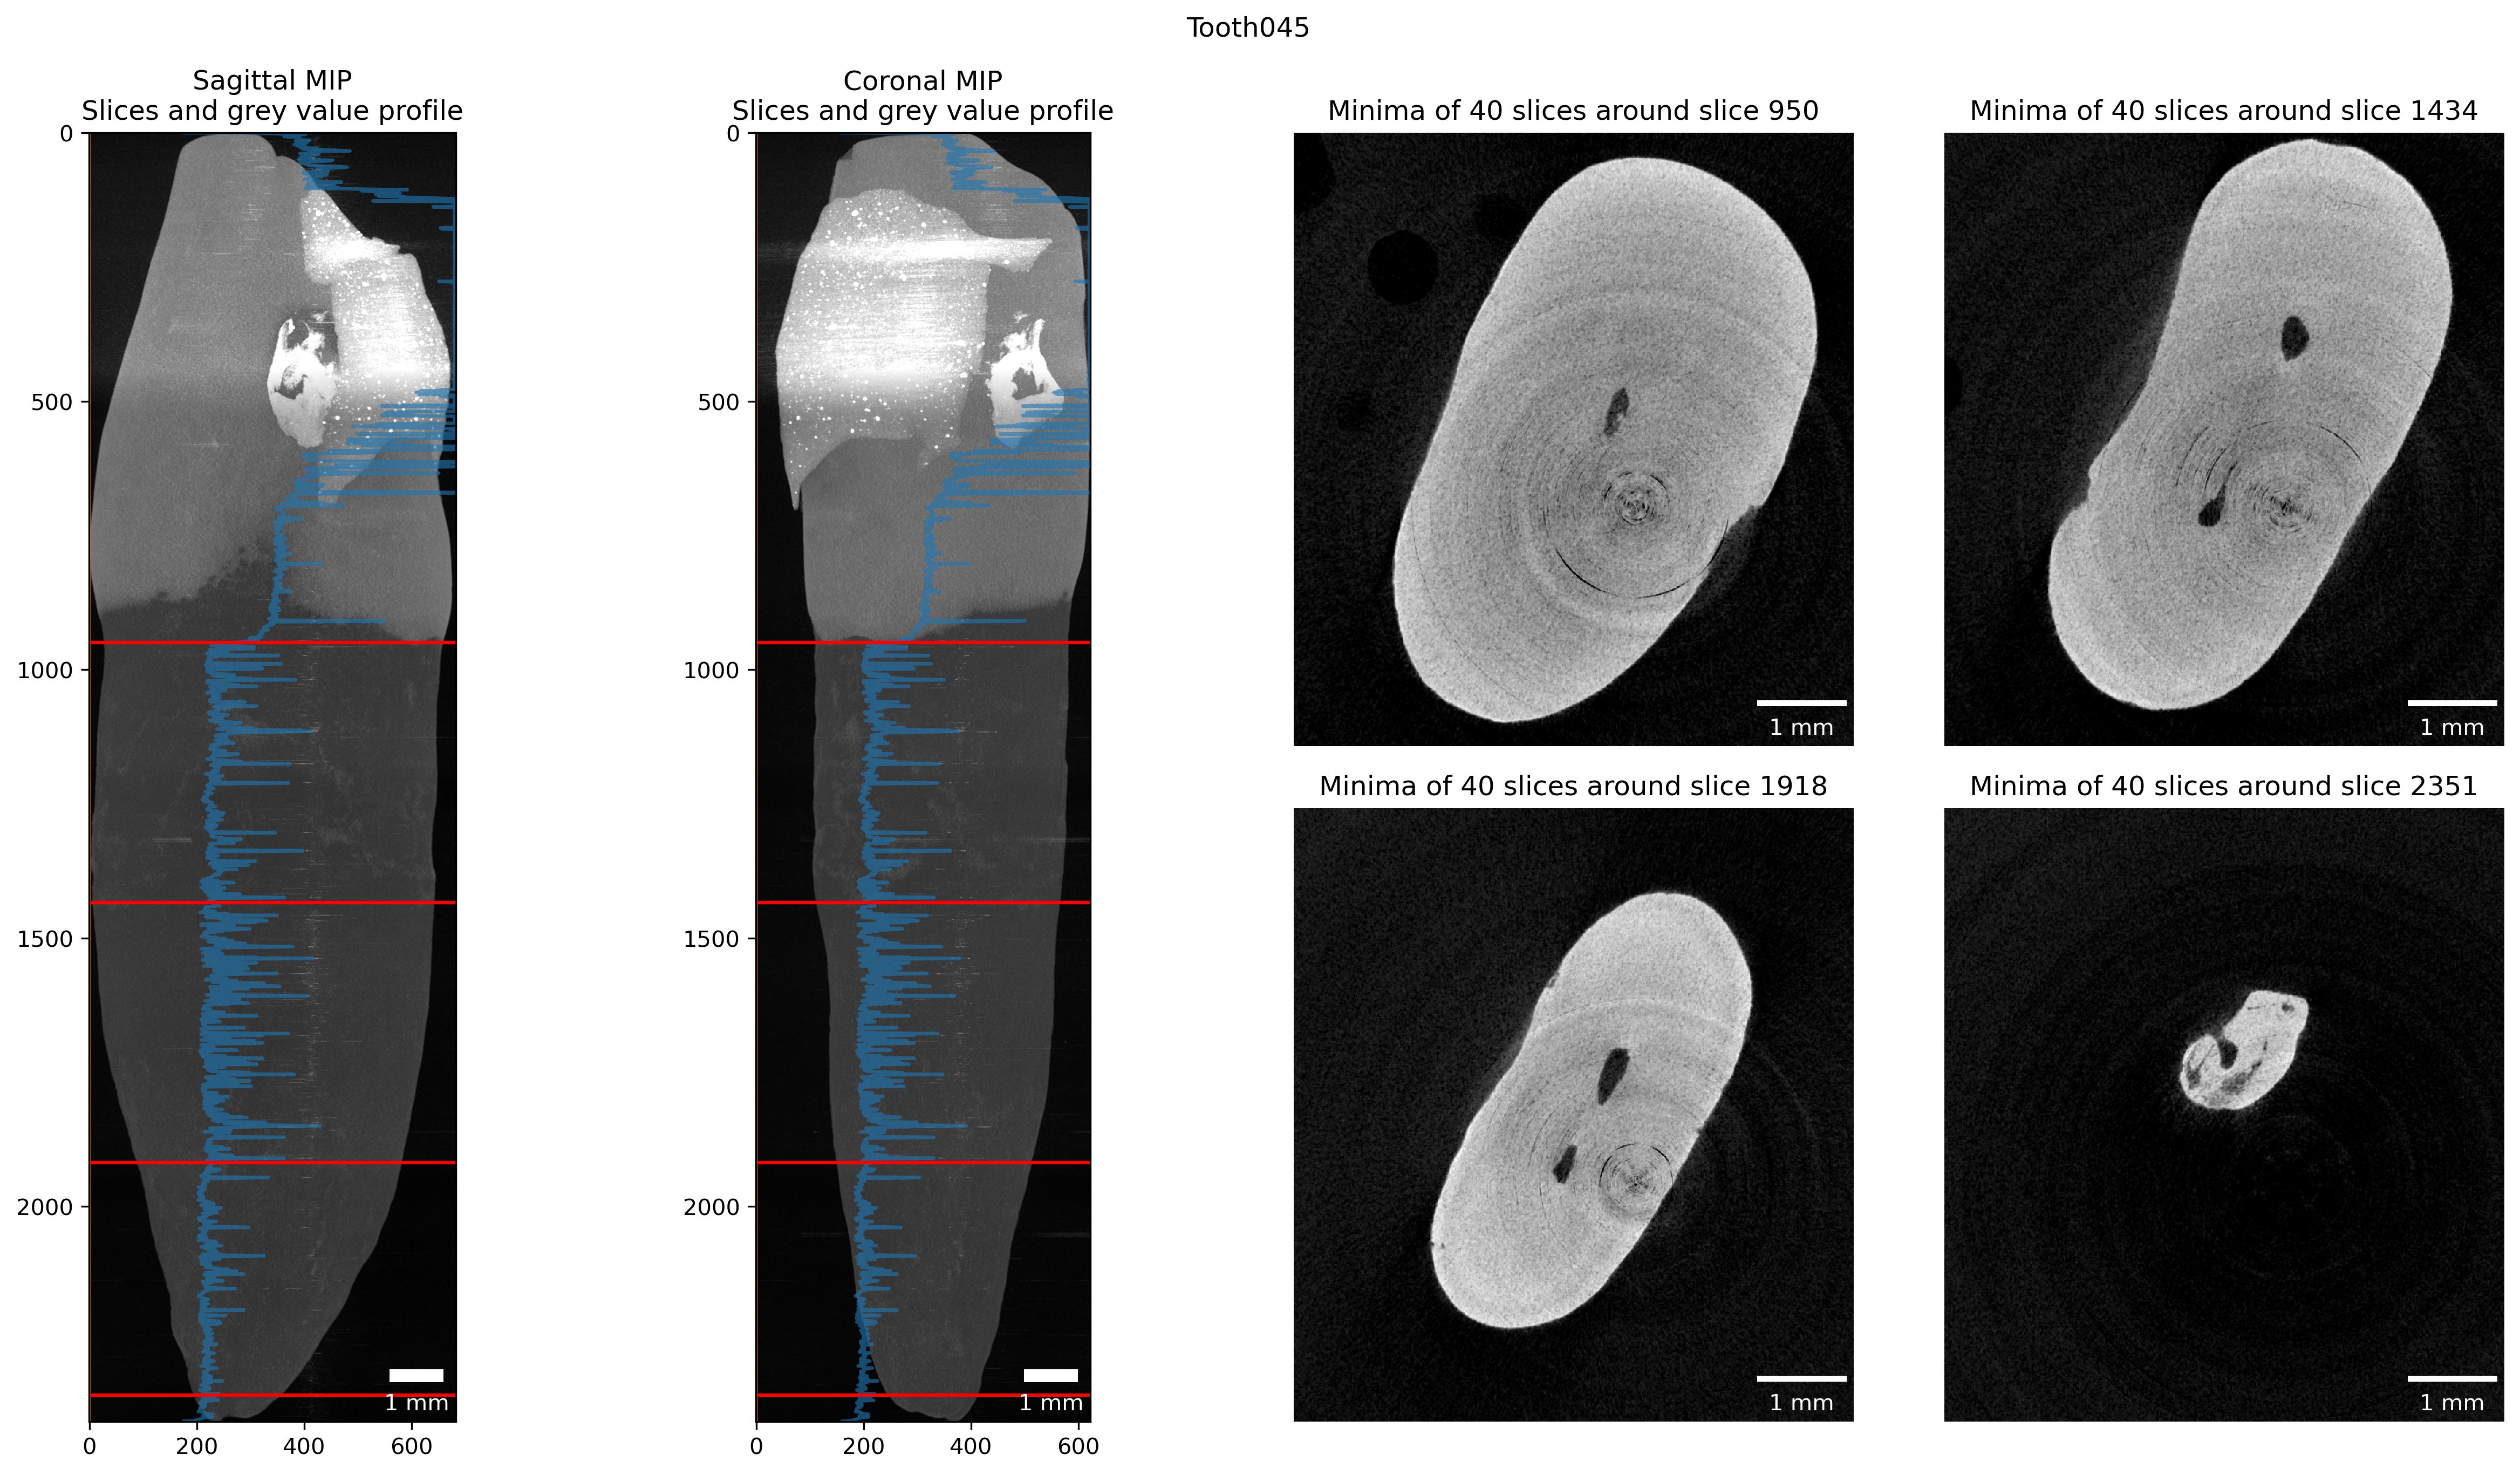
\includegraphics[height=\imageheight]{./images/zmk/tooth045/Tooth045.ExtractedSlices.png}%
		}%
	\only<2|handout:2>{%
		\includegraphics[width=\imagewidth]{./images/zmk/tooth045/Tooth045.Briseno.png}%
		}%
\end{frame}

\begin{frame}
	\frametitle{Classification of root canal configurations}%
	\centering%
	\small{% Smaller text for fitting the table onto the slide
	  \only<1>{%
		\begin{tabular}{llcSS}%
		  \toprule%
		  \multicolumn{2}{c}{Roots} & RCC & \# & \% \\%
		  \midrule%
		  \multicolumn{2}{c}{\multirow{9}{*}{Single (N=98)}}    & 1-1-1/1 & 73 & 74.5\\%
		  \multicolumn{2}{l}{} & 1-1-1/2 & 14 & 14.3\\%
		  \multicolumn{2}{l}{} & 1-1-1/3 & 1 & 1.0\\%
		  \multicolumn{2}{l}{} & 1-1-1/4 & 2 & 2.1\\%
		  \multicolumn{2}{l}{} & 1-1-2/1 & 1 & 1.0\\%
		  \multicolumn{2}{l}{} & 1-2-1/1 & 4 & 4.1\\%
		  \multicolumn{2}{l}{} & 1-2-1/2 & 1 & 1.0\\%
		  \multicolumn{2}{l}{} & 1-2-2/2 & 1 & 1.0\\%
		  \multicolumn{2}{l}{} & 2-3-1/1 & 1 & 1.0\\%
		  \midrule%
		  \multirow{4}{*}{Double (N=3)}  & \multirow{2}{*}{Buccal}  & 1-1-1/1 & 2 & 66.6\\%
		  & & 1-2-1/1 & 1 & 33.3\\%
		  & \multirow{2}{*}{Lingual}  & 1-1-1/1 & 2 & 66.6\\%
		  & & 1-1-1/2 & 1 & 33.3\\%
		  \bottomrule%
		\end{tabular}%
	  }%
	  \only<2|handout:0>{%
		\begin{tabular}{llcSS}%
		  \toprule%
		  \multicolumn{2}{c}{Roots} & RCC & \# & \% \\%
		  \midrule%
		  \multicolumn{2}{c}{\multirow{9}{*}{Single (N=98)}} & 1-1-1/1 & 73 & \cellcolor{ubRed!61.8}74.5\\%
		  \multicolumn{2}{l}{} & 1-1-1/2 & 14 & \cellcolor{ubRed!61.8}14.3\\%
		  \multicolumn{2}{l}{} & 1-1-1/3 & 1 & 1.0\\%
		  \multicolumn{2}{l}{} & 1-1-1/4 & 2 & 2.1\\%
		  \multicolumn{2}{l}{} & 1-1-2/1 & 1 & 1.0\\%
		  \multicolumn{2}{l}{} & 1-2-1/1 & 4 & 4.1\\%
		  \multicolumn{2}{l}{} & 1-2-1/2 & 1 & 1.0\\%
		  \multicolumn{2}{l}{} & 1-2-2/2 & 1 & 1.0\\%
		  \multicolumn{2}{l}{} & 2-3-1/1 & 1 & 1.0\\%
		  \midrule%
		  \multirow{4}{*}{Double (N=3)}  & \multirow{2}{*}{Buccal}    & 1-1-1/1 & 2 & 66.6\\%
		  & & 1-2-1/1 & 1 & 33.3\\%
		  & \multirow{2}{*}{Lingual} & 1-1-1/1 & 2 & 66.6\\%
		  & & 1-1-1/2 & 1 & 33.3\\%
		  \bottomrule%
		\end{tabular}%
	  }%
	}%
\end{frame}%

\begin{frame}
	\frametitle{Extraction of root canal space}
	\begin{tikzpicture}[remember picture,overlay]%
	\node at (current page.center) [shift={(0,-2.9mm)}]{%
		\only<1|handout:0>{%
			\mode<beamer>{%
				\animategraphics[autoplay,loop,width=\paperwidth,every=\everyframe]{24}{./movies/tooth045/transparent-slices/image0}{000}{473}%
				}%
			\mode<handout>{%
				\includegraphics[width=\paperwidth]{./movies/tooth045/transparent-slices/image0000}%
				}%
			}%
		\only<2|handout:1>{%
			\mode<beamer>{%
				\animategraphics[autoplay,loop,width=\paperwidth,every=\everyframe]{24}{./movies/tooth045/transparent-slices-rcs/image0}{000}{457}%
				}%
			\mode<handout>{%
				\includegraphics[width=\paperwidth]{./movies/tooth045/transparent-slices-rcs/image0000}%
				}%
			}%
		\only<3|handout:0>{%
			\mode<beamer>{%
				\animategraphics[autoplay,loop,width=\paperwidth,every=\everyframe]{24}{./movies/tooth045/rcs/image0}{000}{413}%
				}%
			\mode<handout>{%
				\includegraphics[width=\paperwidth]{./movies/tooth045/rcs/image0000}%
				}%
			}%
		};%
	\end{tikzpicture}%
\end{frame}

\begin{frame}
	\renewcommand{\imagewidth}{0.14\linewidth}% 720/2008
	\frametitle{Results of root canal space extraction}%
	\centering%
	\includegraphics[width=\imagewidth]{./images/zmk/rcs/Tooth0452}\hfill%
	\includegraphics[width=\imagewidth]{./images/zmk/rcs/Tooth0278}\hfill%
	\includegraphics[width=\imagewidth]{./images/zmk/rcs/Tooth0353}\hfill%
	\includegraphics[width=\imagewidth]{./images/zmk/rcs/Tooth0419}\hfill%
	\includegraphics[width=\imagewidth]{./images/zmk/rcs/Tooth0642}\hfill%
	\includegraphics[width=\imagewidth]{./images/zmk/rcs/Tooth0752}\hfill%
	% Measuring the tooth length on Tooth093_rec_spr.bmp gives us 2092 pixels. We scanned at 10um.
	% "python ~/P/Dev/latex/draw_a_scalebar.py -i Tooth0931.png -l 2092 -p 10" gives us a scale bar
	\pgfmathsetlength{\imagescale}{\imagewidth/720}%
	\def\x{72}% scalebar-x starting at golden ratio of image width of 720px = 445
	\def\y{1807}% scalebar-y at 90% of image height of 2008px = 1807
	\begin{tikzpicture}[x=\imagescale,y=-\imagescale]
	  \node[anchor=north west, inner sep=0pt, outer sep=0pt] at (0,0) {\includegraphics[width=\imagewidth]{./images/zmk/rcs/Tooth0931}};
	  % 1760.469px = 20.92mm -> 100px = 1188.319um -> 42.076px = 500um, 8.415px = 100um
	  %\draw[|-|,blue,thick] (300,105) -- (327,1865) node [sloped,midway,above,fill=white,semitransparent,text opacity=1] {\qty{20.92}{\milli\meter} (1760px) TEMPORARY!};
	  \draw[|-|,white,shadowed] (\x,\y) -- (\x+420.76,\y) node [midway,above] {\shadowtext{\qty{5}{\milli\meter}}};
	\end{tikzpicture}%
\end{frame}

\begin{frame}
	\frametitle{Physiological foramen geometry}
	\centering%
	\only<1|handout:1>{%
		\includegraphics[height=\imageheight]{./images/zmk/foramen}%
		\sourcecite{Wolf2017}{Fig.~1}%
		}%
	\only<2|handout:0>{%
		\mode<beamer>{%
			\animategraphics[palindrome,autoplay,height=\imageheight,every=\everyframe]{24}{./movies/tooth045/edt-axial/Tooth045_EDT_Axial_}{100}{199}%
			}%
		\mode<handout>{%
			\includegraphics[height=\imageheight]{./movies/tooth045/edt-axial/Tooth045_EDT_Axial_151}%
			}%
		}%
	\only<3|handout:2>{%
		\mode<beamer>{%
			\animategraphics[palindrome,autoplay,height=\imageheight,every=\everyframe]{24}{./movies/tooth045/edt-coronal/Tooth045_EDT_Coronal_}{123}{213}%
			}%
		\mode<handout>{%
			\includegraphics[height=\imageheight]{./movies/tooth045/edt-coronal/Tooth045_EDT_Coronal_139}%
			}%
		}%
\end{frame}

\begin{frame}
	\frametitle{Conclusion ZMK}
	\begin{itemize}
		\item Efficient use of time, \eg more teeth does not mean more (human) work
		\item Reproducible analysis with \emph{free and open-source} software, usable by \emph{anyone}
		\item Objective analysis, \eg no operator bias
	\end{itemize}
\end{frame}

\subsection{Metal foam analysis}
\begin{frame}
	\renewcommand{\imagewidth}{\paperheight}%
	\frametitle{Metal foam}
	\centering%
	\pgfmathsetlength{\imagescale}{\imagewidth/800}%
	\def\x{494}% scalebar-x starting at golden ratio of image width of 800px = 494
	\def\y{540}% scalebar-y at 90% of image height of 600px = 540
	\only<1|handout:1>{%
		\begin{tikzpicture}[x=\imagescale,y=-\imagescale]%
		\node[anchor=north west, inner sep=0pt, outer sep=0pt] at (0,0) {\includegraphics[width=\imagewidth]{./movies/metal_foam/HART_0.4um_Al0.25mm_180_rec_frames/HART_0.4um_Al0.25mm_180_rec0000}};
	%		% 665.634px = 1.221973872mm -> 100px = 183.580um -> 272.360px = 500um, 54.472px = 100um
	%		%\draw[|-|,blue,thick] (67,245) -- (732,237) node [sloped,midway,above,fill=white,semitransparent,text opacity=1] {\qty{1.221973872}{\milli\meter} (666px) TEMPORARY!};
			\draw[|-|,white,shadowed] (\x,\y) -- (\x+272.360,\y) node [midway,above] {\shadowtext{\qty{500}{\micro\meter}}};
		\end{tikzpicture}%
	}%
	\only<2|handout:0>{%
		\animategraphics[autoplay,width=\imagewidth,every=\everyframe]{24}{./movies/metal_foam/HART_0.4um_Al0.25mm_180_rec_frames/HART_0.4um_Al0.25mm_180_rec0}{000}{134}%
	}%
	\only<3|handout:0>{%
		\animategraphics[autoplay,width=\imagewidth,every=\everyframe]{24}{./movies/metal_foam/HART_0.4um_Al0.25mm_180_rec_frames/HART_0.4um_Al0.25mm_180_rec0}{135}{155}%
	}%
	\only<4|handout:0>{%
		\animategraphics[autoplay,width=\imagewidth,every=\everyframe]{24}{./movies/metal_foam/HART_0.4um_Al0.25mm_180_rec_frames/HART_0.4um_Al0.25mm_180_rec0}{156}{239}%
	}%
	\source{Etienne Berner}{NanoElectroCatalysis Group}
\end{frame}

\subsection{A study on fish}
\begin{frame}
	\frametitle{Data wrangling by example: Cichlids}
	\begin{columns}
		\begin{column}{0.6\linewidth}
			Collaboration with team of \href{https://www.aqua.iee.unibe.ch/}{\emph{Aquatic Ecology \& Evolution}}, from the \href{https://www.iee.unibe.ch/}{Institute of Ecology and Evolution}~\footcite{Haberthuer2023}
			\begin{itemize}
				\item 133 Cichlids from Lake Victoria, East Africa
				\begin{itemize}
					\item Functional anatomy of the skulls and jaws
					\item \qtyrange{6}{18}{\centi\meter} in size
				\end{itemize}
				\item 375 scans in total
				\begin{itemize}
					\item Voxelsizes from \qtyrange{3.5}{50}{\micro\meter}
					\item 46 days of scanning time
					\item \qty{9.8}{\tera\byte} of raw data
					\item \qty{1.5}{\tera\byte}/+\num{1000000} reconstructions
				\end{itemize}
			\end{itemize}
		\end{column}
		\begin{column}{0.4\linewidth}
			\centering%
			\only<1|handout:1>{%
				\includegraphics[width=\imagewidth]{./images/cichlids/journal.pone.0291003.g001.png}%
				\sourcelink{https://doi.org/10.1371/journal.pone.0291003.g001}{DOI:gsst8t}{Fig.~1}%
				}%
			\only<2|handout:0>{%
				\lstinputlisting[linerange={2-4,6-7,14-14,16-18,26-30,32-32,36-38,41-42,45-45,55-55}]{./movies/EAWAG/104016/head/proj/104016.log}
				}%
			\only<3|handout:0>{%
				\lstinputlisting[linerange={2-4,6-7,14-14,17-19,26-30,32-32,36-38,41-41,45-45,55-55},
					linebackgroundcolor={\lstcolorlines[ubRed!61.8]{5,6,10,11,15}}]{./movies/EAWAG/104016/head/proj/104016.log}
				}%
			\only<4|handout:0>{%
				\lstinputlisting[linerange={2-4,6-7,14-14,17-19,26-29,31-31,36-38,40-40,45-45},
					linebackgroundcolor={\lstcolorlines[ubRed!61.8]{5,6,10,11,14}}]{./movies/EAWAG/104016/pharynx/proj/104016.log}
				}%
		\end{column}
	\end{columns}
\end{frame}

\begin{frame}
	\renewcommand{\imagewidth}{0.9\linewidth}%
	\frametitle{Visualization of cichlid head}%
	\centering%
	% Generate animations in ImageJ with 3Dscript (files are in repository)
	% Save out as .tif slices
	% mogrify -format png -transparent "rgb(255,255,255)" -fuzz 4% *.tif
	\only<1|handout:1>{%
		\pgfmathsetlength{\imagescale}{\imagewidth/1280}%
		\def\x{791}% scalebar-x starting at golden ratio of image width of 1280px = 791
		\def\y{648}% scalebar-y at 90% of image height of 720px = 648
		\begin{tikzpicture}[x=\imagescale,y=-\imagescale]%
			\node[anchor=north west, inner sep=0pt, outer sep=0pt] at (0,0) {\includegraphics[width=\imagewidth]{./movies/EAWAG/animation.head/104016.head.rec.animation.0000.png}};%
			% 196.739px = 6.045mm -> 100px = 3072.594um -> 16.273px = 500um, 3.255px = 100um
			\draw[|-|,white,shadowed] (652,353) -- (849,369) node [sloped,midway,above] {\shadowtext{\(\approx\)\SI{6}{\milli\meter}}};%
		\end{tikzpicture}%
	}%
	\only<2|handout:2>{%
		% Show PJ
		\mode<beamer>{\animategraphics[autoplay,width=\imagewidth,every=\everyframe]{24}{./movies/EAWAG/animation.head/104016.head.rec.animation.0}{000}{480}}%
		\mode<handout>{\includegraphics[width=\imagewidth]{./movies/EAWAG/animation.head/104016.head.rec.animation.0480}}%
	}%
	\only<3|handout:0>{%
		% Show full head again
		\animategraphics[autoplay,width=\imagewidth,every=\everyframe]{24}{./movies/EAWAG/animation.head/104016.head.rec.animation.}{0481}{0960}%
	}%
	\only<4|handout:0>{%
		% Zoom to otolith
		\animategraphics[autoplay,width=\imagewidth,every=\everyframe]{24}{./movies/EAWAG/animation.head/104016.head.rec.animation.}{0961}{1440}%
	}%
	\only<5|handout:0>{%
		%Move to PJ
		\animategraphics[autoplay,width=\imagewidth,every=\everyframe]{24}{./movies/EAWAG/animation.head/104016.head.rec.animation.}{1441}{1920}%
	}%
	\note[item]<1>{Fish 104016, Scan head\_rec; This fish was scanned on 2022-01-27T13:32:59 on the SkyScan2214, with a voxel size of \qty{13.0}{\micro\meter}.}%
	\note[item]<1>{The eye has a diameter of approximately \qty{6}{\milli\meter}.}%
	\note[item]<1>{DOI:10.1002/ece3.9669: The detritivorous Enterochromis cinctus Greenwood \& Gee, 1969 has a red dorsum and a bright yellow flank too but it has dark vertical bars and lacks any mid-lateral band.%
		Before the near extinctions, it used to occur at depths between \qtyrange{13}{60}{\meter} (Greenwood \& Gee, 1969).}%
\end{frame}

\begin{frame}
	\renewcommand{\imagewidth}{0.9\linewidth}%
	\frametitle{Visualization of segmented pharyngeal jaw}%
	\centering%
	\only<1|handout:0>{%
		%Animate from head-dataset to segmented pj
		\animategraphics[autoplay,width=\imagewidth,every=\everyframe]{24}{./movies/EAWAG/animation.head2pj/morphed.0}{000}{240}%
		}%
	\only<2|handout:1>{%
		\pgfmathsetlength{\imagescale}{\imagewidth/1280}%
		\def\x{791}% scalebar-x starting at golden ratio of image width of 1280px = 791
		\def\y{648}% scalebar-y at 90% of image height of 720px = 648
		\begin{tikzpicture}[x=\imagescale,y=-\imagescale]%
			\node[anchor=north west, inner sep=0pt, outer sep=0pt] at (0,0) {\includegraphics[width=\imagewidth]{./movies/EAWAG/animation.pj/104016.pj.animation.0000.png}};%
			% 846.456px = 4.9mm -> 100px = 578.885um -> 86.373px = 500um, 17.275px = 100um
			\draw[|-|,white,shadowed] (209,23) -- (1055,26) node [sloped,midway,below] {\shadowtext{\(\approx\)\SI{5}{\milli\meter}}};%
		\end{tikzpicture}%
  	}%
	\only<3|handout:0>{%
		\animategraphics[autoplay,width=\imagewidth,every=\everyframe]{24}{./movies/EAWAG/animation.pj/104016.pj.animation.0}{000}{700}%
	}%
	\only<4|handout:0>{%
		\animategraphics[autoplay,width=\imagewidth,every=\everyframe]{24}{./movies/EAWAG/animation.pj/104016.pj.animation.}{0701}{1440}%
	}%
	\note[item]<1|handout:1>{Fish 104016, Scan pharynx\_rec; This fish was scanned on 2021-02-04T13:30:11 on the SkyScan1272, with a voxel size of \qty{5.0}{\micro\meter}.}%
	\note[item]<1|handout:1>{The distance between the two ends at the top is approximately \qty{5}{\milli\meter}.}%
	\note[item]<1|handout:1>{A human hair typically has a thickness ranging from \qtyrange{17}{181}{\micro\meter}, depending on various factors like the individual's hair type, age, and ethnicity. On average, most human hair strands fall between \qtyrange{50}{100}{\micro\meter} in diameter.}%
\end{frame}

\begin{frame}
	\frametitle{Data wrangling by example: Cichlids}
	\centering%
	\includegraphics<1|handout:0>[width=\imagewidth]{./images/cichlids/Otolither_104016_head_01_Overview}%
	\includegraphics<2|handout:0>[width=\imagewidth]{./images/cichlids/Otolither_104016_head_02_GrayValues}%
	\includegraphics<3|handout:0>[width=\imagewidth]{./images/cichlids/Otolither_104016_head_03_GrayValuesRegion}%
	\includegraphics<4|handout:1>[width=\imagewidth]{./images/cichlids/Otolither_104016_head_04_GrayValuesSmoothed}%
	\includegraphics<5|handout:0>[width=\imagewidth]{./images/cichlids/Otolither_104016_head_05_Peaks}%
	\includegraphics<6|handout:0>[width=\imagewidth]{./images/cichlids/Otolither_104016_head_06_Peaks_All}%
	\includegraphics<7|handout:0>[width=\imagewidth]{./images/cichlids/Otolither_104016_head_07_ExtractedRegions}%
	\includegraphics<8|handout:0>[width=\imagewidth]{./images/cichlids/Otolither_104016_head_08_ExtractedRegionsMIPs}%
	\includegraphics<9|handout:2>[width=\imagewidth]{./images/cichlids/Otolither_104016_head_09_ExtractedOtolithMasked}%
	\only<10|handout:0>{\href{https://htmlpreview.github.io/?https://github.com/habi/EAWAG-manuscript/blob/main/content/data/104016_Enterochromis_I_cinctus_St_E.head.rec.Otolith.Region.3D.html}{Exported 3D view}}%
\end{frame}

\begin{frame}%
	\frametitle{Thanks!}%
	\begin{itemize}%
		\item Thanks for listening to me!%
		\item<2-> \href{https://mannerofspeaking.org/2019/12/29/what-questions-do-you-have-for-me/}{What questions do you have for me?}%
	\end{itemize}%
	\only<3|handout:0>{%
		\begin{tikzpicture}[remember picture,overlay]%
			\node at (current page.center) {%
				\animategraphics[loop,autoplay,width=\paperwidth,every=\everyframe]{24}{./movies/mouse_skull/mouse_skull}{000}{236}%
				};%
		\end{tikzpicture}%
	}%
\end{frame}

\begin{frame}
	\frametitle{\href{https://en.wikipedia.org/wiki/Colophon_(publishing)}{Colophon}}
	\begin{itemize}
	  \item This \textsc{beamer} presentation was crafted in \LaTeX\xspace with the (slightly adapted) \href{http://intern.unibe.ch/dienstleistungen/corporate_design_und_vorlagen/praesentationen/}{template from \emph{Corporate Design und Vorlagen} of the University of Bern}.
		\begin{itemize}
		  \item \href{https://github.com/habi/lecture.microtomography/}{Complete source code: git.io/fjpP7}
		  \item The \LaTeX\xspace code is automatically compiled with a \href{https://github.com/actions}{GitHub action} to a \href{https://habi.github.io/Lecture.Microtomography/XRayMicroTomography.Handout.pdf}{(handout) PDF which you can access here: git.io/JeQxO}
		\end{itemize}
	  \item Did you spot an error?
		\begin{itemize}
		  \item \href{https://github.com/habi/lecture.microtomography/issues}{File an issue: git.io/fjpPb}
		  \item \href{https://github.com/habi/lecture.microtomography/pulls}{Submit a pull request: git.io/fjpPN}
		  \item \href{mailto:david.haberthuer@unibe.ch?subject=Error\%20in\%20the\%20(micro)-tomography\%20lecture\&body=https://xkcd.com/386/}{Send me an email: david.haberthuer@unibe.ch}
		\end{itemize}
	\end{itemize}
  \end{frame}

\begin{frame}[allowframebreaks]
	\frametitle{References}
	\renewcommand*{\bibfont}{\footnotesize}%
	\printbibliography%
\end{frame}

\end{document}
